%!TeX spellcheck = hu_HU
% !TeX encoding = UTF-8
% !TeX program = xelatex
% TODO Change language to en_GB (recommended) or en_US for English documents
\documentclass[11pt,a4paper,oneside]{report}             % Single-side
%\documentclass[11pt,a4paper,twoside,openright]{report}  % Duplex

% thanks to http://tex.stackexchange.com/a/47579/71109
\usepackage{ifxetex}
\usepackage{ifluatex}
\newif\ifxetexorluatex % a new conditional starts as false
\ifnum 0\ifxetex 1\fi\ifluatex 1\fi>0
   \xetexorluatextrue
\fi

\ifxetexorluatex
  \usepackage{fontspec}
\else
  \usepackage[T1]{fontenc}
  \usepackage[utf8]{inputenc}
  \usepackage[lighttt]{lmodern}
\fi

\usepackage[english,magyar]{babel} % Alapértelmezés szerint utoljára definiált nyelv lesz aktív, de később külön beállítjuk az aktív nyelvet.

%\usepackage{cmap}
\usepackage{amsfonts,amsmath,amssymb} % Mathematical symbols.
%\usepackage[ruled,boxed,resetcount,linesnumbered]{algorithm2e} % For pseudocodes. % beware: this is not compatible with LuaLaTeX, see http://tex.stackexchange.com/questions/34814/lualatex-and-algorithm2e
\usepackage{booktabs} % For publication quality tables for LaTeX
\usepackage{graphicx}

%\usepackage{fancyhdr}
%\usepackage{lastpage}

\usepackage{anysize}
%\usepackage{sectsty}
\usepackage{setspace} % For setting line spacing

\usepackage[unicode]{hyperref} % For hyperlinks in the generated document.
\usepackage{xcolor}
\usepackage{listings} % For source code snippets.

\usepackage[amsmath,thmmarks]{ntheorem} % Theorem-like environments.

\usepackage[hang]{caption}

\singlespacing

\newcommand{\selecthungarian}{
	\selectlanguage{magyar}
	\setlength{\parindent}{2em}
	\setlength{\parskip}{0em}
	\frenchspacing
}

\newcommand{\selectenglish}{
	\selectlanguage{english}
	\setlength{\parindent}{0em}
	\setlength{\parskip}{0.5em}
	\nonfrenchspacing
	\renewcommand{\figureautorefname}{Figure}
	\renewcommand{\tableautorefname}{Table}
	\renewcommand{\partautorefname}{Part}
	\renewcommand{\chapterautorefname}{Chapter}
	\renewcommand{\sectionautorefname}{Section}
	\renewcommand{\subsectionautorefname}{Section}
	\renewcommand{\subsubsectionautorefname}{Section}
}

\usepackage[numbers]{natbib}
\usepackage{xspace}

\usepackage{xparse,nameref}
\usepackage{tikz}
\usetikzlibrary{shapes,calc}
\usetikzlibrary{positioning}
\usetikzlibrary{decorations.markings}
\usepackage{float}
\linespread{1.5}
\marginsize{35mm}{25mm}{15mm}{15mm}
\usepackage{array}
\newcolumntype{x}[1]{
>{\centering\hspace{0pt}}p{#1}}

\usepackage{pgfplots}
\usepackage{filecontents}
\pgfplotsset{compat=newest}
\usepackage{subcaption}

\usepackage{amsmath}

\usepackage{newtxmath}
\newcommand{\sm}[1]{{\scriptscriptstyle#1}}

%TODO Set the main variables
\newcommand{\vikszerzoVezeteknev}{Bánóczi}
\newcommand{\vikszerzoKeresztnev}{Dávid}

\newcommand{\vikkonzulensAMegszolitas}{dr.~}
\newcommand{\vikkonzulensAVezeteknev}{Hullám}
\newcommand{\vikkonzulensAKeresztnev}{Gábor}

\newcommand{\vikkonzulensBMegszolitas}{}
\newcommand{\vikkonzulensBVezeteknev}{}
\newcommand{\vikkonzulensBKeresztnev}{}

\newcommand{\vikkonzulensCMegszolitas}{}
\newcommand{\vikkonzulensCVezeteknev}{}
\newcommand{\vikkonzulensCKeresztnev}{}

\newcommand{\vikcim}{Magyarázat generálás mély neurális háló alapú osztályozáshoz} % Cím
\newcommand{\viktanszek}{\bmemit} % Tanszék
\newcommand{\vikdoktipus}{\bsc} % Dokumentum típusa (\bsc vagy \msc)
\newcommand{\vikmunkatipusat}{szakdolgozatot} % a "hallgató nyilatkozat" részhez: szakdolgozatot vagy diplomatervet

%--------------------------------------------------------------------------------------
% TDK-specifikus változók
%--------------------------------------------------------------------------------------
\newcommand{\tdkszerzoB}{Második Szerző} % Második szerző neve; hagyd üresen, ha egyedül írtad a TDK-t.
\newcommand{\tdkev}{2014} % A dolgozat írásának éve (pl. "2014") (Ez OTDK-nál eltérhet az aktuális évtől.)

% További adatok az OTDK címlaphoz (BME-s TDK-hoz nem kell kitölteni)
\newcommand{\tdkevfolyamA}{IV} % Első szerző évfolyama, római számmal (pl. IV).
\newcommand{\tdkevfolyamB}{III} % Második szerző évfolyama, római számmal (pl. III).
\newcommand{\tdkkonzulensbeosztasA}{egyetemi tanár} % Első konzulens beosztása (pl. egyetemi docens)
\newcommand{\tdkkonzulensbeosztasB}{doktorandusz} % Második konzulens beosztása (pl. egyetemi docens)

\newcommand{\szerzoMeta}{\vikszerzoVezeteknev{} \vikszerzoKeresztnev} % egy szerző esetén
%\newcommand{\szerzoMeta}{\vikszerzoVezeteknev{} \vikszerzoKeresztnev, \tdkszerzoB} % két szerző esetén

%TODO Language configuration -- choose one
% Beállítások magyar nyelvű dolgozathoz
%--------------------------------------------------------------------------------------
% Elnevezések
%--------------------------------------------------------------------------------------
\newcommand{\bme}{Budapesti Műszaki és Gazdaságtudományi Egyetem}
\newcommand{\vik}{Villamosmérnöki és Informatikai Kar}

\newcommand{\bmemit}{Méréstechnika és Információs Rendszerek Tanszék}

\newcommand{\keszitette}{Készítette}
\newcommand{\konzulens}{Konzulens}

\newcommand{\bsc}{Szakdolgozat}
\newcommand{\msc}{Diplomaterv}
\newcommand{\tdk}{TDK dolgozat}
\newcommand{\bsconlab}{BSc Önálló laboratórium}
\newcommand{\msconlabi}{MSc Önálló laboratórium 1.}
\newcommand{\msconlabii}{MSc Önálló laboratórium 2.}

\newcommand{\pelda}{Példa}
\newcommand{\definicio}{Definíció}
\newcommand{\tetel}{Tétel}

\newcommand{\bevezetes}{Bevezetés}
\newcommand{\koszonetnyilvanitas}{Köszönetnyilvánítás}
\newcommand{\fuggelek}{Függelék}

% Opcionálisan átnevezhető címek
%\addto\captionsmagyar{%
%\renewcommand{\listfigurename}{Saját ábrajegyzék cím}
%\renewcommand{\listtablename}{Saját táblázatjegyzék cím}
%\renewcommand{\bibname}{Saját irodalomjegyzék név}
%}

\newcommand{\szerzo}{\vikszerzoVezeteknev{} \vikszerzoKeresztnev}
\newcommand{\vikkonzulensA}{\vikkonzulensAMegszolitas\vikkonzulensAVezeteknev{} \vikkonzulensAKeresztnev}
\newcommand{\vikkonzulensB}{\vikkonzulensBMegszolitas\vikkonzulensBVezeteknev{} \vikkonzulensBKeresztnev}
\newcommand{\vikkonzulensC}{\vikkonzulensCMegszolitas\vikkonzulensCVezeteknev{} \vikkonzulensCKeresztnev}

\newcommand{\selectthesislanguage}{\selecthungarian}

\bibliographystyle{huplain}

\def\lstlistingname{lista}

\newcommand{\appendixnumber}{6}  % a fofejezet-szamlalo az angol ABC 6. betuje (F) lesz

% Settings for English documents
%%--------------------------------------------------------------------------------------
% Elnevezések
%--------------------------------------------------------------------------------------
\newcommand{\bme}{Budapest University of Technology and Economics}
\newcommand{\vik}{Faculty of Electrical Engineering and Informatics}

\newcommand{\bmemit}{Department of Measurement and Information Systems}

\newcommand{\keszitette}{Author}
\newcommand{\konzulens}{Advisor}

\newcommand{\bsc}{Bachelor's Thesis}
\newcommand{\msc}{Master's Thesis}
\newcommand{\tdk}{Scientific Students' Association Report}
\newcommand{\bsconlab}{BSc Project Laboratory}
\newcommand{\msconlabi}{MSc Project Laboratory 1}
\newcommand{\msconlabii}{MSc Project Laboratory 2}

\newcommand{\pelda}{Example}
\newcommand{\definicio}{Definition}
\newcommand{\tetel}{Theorem}

\newcommand{\bevezetes}{Introduction}
\newcommand{\koszonetnyilvanitas}{Acknowledgements}
\newcommand{\fuggelek}{Appendix}

% Optional custom titles
%\addto\captionsenglish{%
%\renewcommand*{\listfigurename}{Your list of figures title}
%\renewcommand*{\listtablename}{Your list of tables title}
%\renewcommand*{\bibname}{Your bibliography title}
%}

\newcommand{\szerzo}{\vikszerzoKeresztnev{} \vikszerzoVezeteknev}
\newcommand{\vikkonzulensA}{\vikkonzulensAMegszolitas\vikkonzulensAKeresztnev{} \vikkonzulensAVezeteknev}
\newcommand{\vikkonzulensB}{\vikkonzulensBMegszolitas\vikkonzulensBKeresztnev{} \vikkonzulensBVezeteknev}
\newcommand{\vikkonzulensC}{\vikkonzulensCMegszolitas\vikkonzulensCKeresztnev{} \vikkonzulensCVezeteknev}

\newcommand{\selectthesislanguage}{\selectenglish}

\bibliographystyle{plainnat}

\newcommand{\ie}{i.e.\@\xspace}
\newcommand{\Ie}{I.e.\@\xspace}
\newcommand{\eg}{e.g.\@\xspace}
\newcommand{\Eg}{E.g.\@\xspace}
\newcommand{\etal}{et al.\@\xspace}
\newcommand{\etc}{etc.\@\xspace}
\newcommand{\vs}{vs.\@\xspace}
\newcommand{\viz}{viz.\@\xspace} % videlicet
\newcommand{\cf}{cf.\@\xspace} % confer
\newcommand{\Cf}{Cf.\@\xspace}
\newcommand{\wrt}{w.r.t.\@\xspace} % with respect to
\newcommand{\approximately}{approx.\xspace}

\newcommand{\appendixnumber}{1}  % a fofejezet-szamlalo az angol ABC 1. betuje (A) lesz


%--------------------------------------------------------------------------------------
% Page layout setup
%--------------------------------------------------------------------------------------
% we need to redefine the pagestyle plain
% another possibility is to use the body of this command without \fancypagestyle
% and use \pagestyle{fancy} but in that case the special pages
% (like the ToC, the References, and the Chapter pages)remain in plane style

\pagestyle{plain}
\marginsize{35mm}{25mm}{15mm}{15mm}

\setcounter{tocdepth}{3}
%\sectionfont{\large\upshape\bfseries}
\setcounter{secnumdepth}{3}

\sloppy % Margón túllógó sorok tiltása.
\widowpenalty=10000 \clubpenalty=10000 %A fattyú- és árvasorok elkerülése
\def\hyph{-\penalty0\hskip0pt\relax} % Kötőjeles szavak elválasztásának engedélyezése


%--------------------------------------------------------------------------------------
% Setup hyperref package
%--------------------------------------------------------------------------------------
\hypersetup{
    % bookmarks=true,            % show bookmarks bar?
    unicode=true,              % non-Latin characters in Acrobat's bookmarks
    pdftitle={\vikcim},        % title
    pdfauthor={\szerzoMeta},    % author
    pdfsubject={\vikdoktipus}, % subject of the document
    pdfcreator={\szerzoMeta},   % creator of the document
    pdfproducer={},    % producer of the document
    pdfkeywords={},    % list of keywords (separate then by comma)
    pdfnewwindow=true,         % links in new window
    colorlinks=true,           % false: boxed links; true: colored links
    linkcolor=black,           % color of internal links
    citecolor=black,           % color of links to bibliography
    filecolor=black,           % color of file links
    urlcolor=black             % color of external links
}


%--------------------------------------------------------------------------------------
% Set up listings
%--------------------------------------------------------------------------------------
\definecolor{lightgray}{rgb}{0.95,0.95,0.95}
\lstset{
	basicstyle=\scriptsize\ttfamily, % print whole listing small
	keywordstyle=\color{black}\bfseries, % bold black keywords
	identifierstyle=, % nothing happens
	% default behavior: comments in italic, to change use
	% commentstyle=\color{green}, % for e.g. green comments
	stringstyle=\scriptsize,
	showstringspaces=false, % no special string spaces
	aboveskip=3pt,
	belowskip=3pt,
	backgroundcolor=\color{lightgray},
	columns=flexible,
	keepspaces=true,
	escapeinside={(*@}{@*)},
	captionpos=b,
	breaklines=true,
	frame=single,
	float=!ht,
	tabsize=2,
	literate=*
		{á}{{\'a}}1	{é}{{\'e}}1	{í}{{\'i}}1	{ó}{{\'o}}1	{ö}{{\"o}}1	{ő}{{\H{o}}}1	{ú}{{\'u}}1	{ü}{{\"u}}1	{ű}{{\H{u}}}1
		{Á}{{\'A}}1	{É}{{\'E}}1	{Í}{{\'I}}1	{Ó}{{\'O}}1	{Ö}{{\"O}}1	{Ő}{{\H{O}}}1	{Ú}{{\'U}}1	{Ü}{{\"U}}1	{Ű}{{\H{U}}}1
}


%--------------------------------------------------------------------------------------
% Set up theorem-like environments
%--------------------------------------------------------------------------------------
% Using ntheorem package -- see http://www.math.washington.edu/tex-archive/macros/latex/contrib/ntheorem/ntheorem.pdf

\theoremstyle{plain}
\theoremseparator{.}
\newtheorem{example}{\pelda}

\theoremseparator{.}
%\theoremprework{\bigskip\hrule\medskip}
%\theorempostwork{\hrule\bigskip}
\theorembodyfont{\upshape}
\theoremsymbol{{\large \ensuremath{\centerdot}}}
\newtheorem{definition}{\definicio}

\theoremseparator{.}
%\theoremprework{\bigskip\hrule\medskip}
%\theorempostwork{\hrule\bigskip}
\newtheorem{theorem}{\tetel}


%--------------------------------------------------------------------------------------
% Some new commands and declarations
%--------------------------------------------------------------------------------------
\newcommand{\code}[1]{{\upshape\ttfamily\scriptsize\indent #1}}
\newcommand{\doi}[1]{DOI: \href{http://dx.doi.org/\detokenize{#1}}{\raggedright{\texttt{\detokenize{#1}}}}} % A hivatkozások közt így könnyebb DOI-t megadni.

\DeclareMathOperator*{\argmax}{arg\,max}
%\DeclareMathOperator*[1]{\floor}{arg\,max}
\DeclareMathOperator{\sign}{sgn}
\DeclareMathOperator{\rot}{rot}


%--------------------------------------------------------------------------------------
% Setup captions
%--------------------------------------------------------------------------------------
\captionsetup[figure]{
	width=.75\textwidth,
	aboveskip=10pt}

\renewcommand{\captionlabelfont}{\bf}
%\renewcommand{\captionfont}{\footnotesize\it}

%--------------------------------------------------------------------------------------
% Hyphenation exceptions
%--------------------------------------------------------------------------------------
\hyphenation{Shakes-peare Mar-seilles ár-víz-tű-rő tü-kör-fú-ró-gép}


\author{\vikszerzo}
\title{\viktitle}

\DeclareRobustCommand\tikzcircle{\tikz \draw[line width=0.5mm]  circle(0.5ex);}

\DeclareRobustCommand\tikzrectangle{\tikz \draw[line width=0.5mm] (0ex,0ex)  rectangle ++(1ex,1ex);}


%--------------------------------------------------------------------------------------
% Table of contents and the main text
%--------------------------------------------------------------------------------------
\begin{document}

\NewDocumentCommand{\chapref}{s m}{\aref{#2}.~Fejezet~}

\pagenumbering{gobble}
%--------------------------------------------------------------------------------------
% Feladatkiiras (a tanszeken atveheto, kinyomtatott valtozat)
%--------------------------------------------------------------------------------------
\clearpage
\begin{center}
\large
\textbf{FELADATKIÍRÁS}\\
\end{center}

A feladatkiírást a tanszéki adminisztrációban lehet átvenni, és a leadott munkába eredeti, tanszéki pecséttel ellátott és a tanszékvezető által aláírt lapot kell belefűzni (ezen oldal \emph{helyett}, ez az oldal csak útmutatás). Az elektronikusan feltöltött dolgozatban már nem kell beleszerkeszteni ezt a feladatkiírást.


\selectthesislanguage

%TODO Titlepage -- choose one from below
%~~~~~~~~~~~~~~~~~~~~~~~~~~~~~~~~~~~~~~~~~~~~~~~~~~~~~~~~~~~~~~~~~~~~~~~~~~~~~~~~~~~~~~
\hypersetup{pageanchor=false}
%--------------------------------------------------------------------------------------
%	The title page
%--------------------------------------------------------------------------------------
\begin{titlepage}
\begin{center}

\includegraphics[width=60mm,keepaspectratio]{figures/bme_logo.pdf}\\
\vspace{0.3cm}
\textbf{\bme}\\
\textmd{\vik}\\
\textmd{\viktanszek}\\[5cm]

\vspace{0.4cm}
{\huge \bfseries \vikcim}\\[0.8cm]
\vspace{0.5cm}
\textsc{\Large \vikdoktipus}\\[4cm]

{
	\renewcommand{\arraystretch}{0.85}
	\begin{tabular}{cc}
	 \makebox[7cm]{\emph{\keszitette}} & \makebox[7cm]{\emph{\konzulens}} \\ \noalign{\smallskip}
	 \makebox[7cm]{\szerzo} & \makebox[7cm]{\vikkonzulensA} \\
	  & \makebox[7cm]{\vikkonzulensB} \\
	  & \makebox[7cm]{\vikkonzulensC} \\
	\end{tabular}
}

\vfill
{\large \today}
\end{center}
\end{titlepage}
\hypersetup{pageanchor=false}

		   % Szakdolgozat/Diplomaterv címlap
%%% TDK címlap
\begin{titlepage}
  \begin{center}  
  
\includegraphics[width=7cm]{./figures/bme_logo.pdf}
  \vspace{0.3cm}
  
  \bme \\
  \vik \\
  \viktanszek \\
  \vspace{5cm}
  
  \huge {\vikcim}
  \vspace{1.5cm}
  
  \large {\textbf{\tdk}}
  \vfill
    
  {\Large 
  	\keszitette: \\ \vspace{0.3cm}
  	\szerzo \\
	\tdkszerzoB \\
  	\vspace{1.5cm}
  	\konzulens: \\ \vspace{0.3cm}
  	\vikkonzulensA \\
  	\vikkonzulensB \\
  }
  
  \vspace{2cm}
  \large {\tdkev}
 \end{center}
\end{titlepage}
%% Címlap vége
	% TDK címlap
%%% OTDK külső címlap
\begin{titlepage}
  	$\;$ 
	\vspace{5cm}
	
	\begin{center}
	\Huge
	\textbf{TDK-dolgozat}\let\thefootnote\relax\footnote{A dolgozat bemutatását a XXXXXXXXX  ``Lorem ipsum dolor sit amet'' című program támogatta.}
	\end{center}
	
	\vspace{13cm}
	
	\Large
	\hspace{8cm} \szerzo
	
	\hspace{8cm} \tdkszerzoB
	
	\hspace{8cm} \tdkev.
\end{titlepage}

\newpage
\thispagestyle{empty}


%% OTDK belső címlap
\begin{titlepage}
  \begin{center}  
  
\includegraphics[width=7cm]{./figures/bme_logo.pdf}
  \vspace{0.3cm}
  
  \bme \\
  \vik \\
  \viktanszek \\
  \vspace{3.5cm}
  
  \huge {\vikcim}
  \vspace{1.5cm}
  
  \large {\textbf{\vikdoktipus}}
  \vfill
    
  {\Large 
  	{\large \keszitette:} \\ \vspace{0.2cm}
  	\szerzo \\ \tdkevfolyamA. évfolyam \\
	\vspace{0.5cm}
	\tdkszerzoB \\ \tdkevfolyamB. évfolyam \\
  	\vspace{1.5cm}
  	{\large \konzulens:} \\ \vspace{0.2cm}
  	\vikkonzulensA,\\ \tdkkonzulensbeosztasA \\
  	\vspace{0.5cm}
  	\vikkonzulensB,\\ \tdkkonzulensbeosztasB \\
  }
  
  \vspace{2cm}
  \large {\tdkev.}
  
 \end{center}
\end{titlepage}   % OTDK címlap


% Table of Contents
%~~~~~~~~~~~~~~~~~~~~~~~~~~~~~~~~~~~~~~~~~~~~~~~~~~~~~~~~~~~~~~~~~~~~~~~~~~~~~~~~~~~~~~
\tableofcontents\vfill


% Declaration and Abstract
%~~~~~~~~~~~~~~~~~~~~~~~~~~~~~~~~~~~~~~~~~~~~~~~~~~~~~~~~~~~~~~~~~~~~~~~~~~~~~~~~~~~~~~
\selectlanguage{magyar}
\pagenumbering{gobble}
%--------------------------------------------------------------------------------------
% Nyilatkozat
%--------------------------------------------------------------------------------------
\begin{center}
\large
\textbf{HALLGATÓI NYILATKOZAT}\\
\end{center}

Alulírott \emph{\vikszerzoVezeteknev{} \vikszerzoKeresztnev}, szigorló hallgató kijelentem, hogy ezt a \vikmunkatipusat{} meg nem engedett segítség nélkül, saját magam készítettem, csak a megadott forrásokat (szakirodalom, eszközök stb.) használtam fel. Minden olyan részt, melyet szó szerint, vagy azonos értelemben, de átfogalmazva más forrásból átvettem, egyértelműen, a forrás megadásával megjelöltem.

Hozzájárulok, hogy a jelen munkám alapadatait (szerző(k), cím, angol és magyar nyelvű tartalmi kivonat, készítés éve, konzulens(ek) neve) a BME VIK nyilvánosan hozzáférhető elektronikus formában, a munka teljes szövegét pedig az egyetem belső hálózatán keresztül (vagy autentikált felhasználók számára) közzétegye. Kijelentem, hogy a benyújtott munka és annak elektronikus verziója megegyezik. Dékáni engedéllyel titkosított diplomatervek esetén a dolgozat szövege csak 3 év eltelte után válik hozzáférhetővé.

\begin{flushleft}
\vspace*{1cm}
Budapest, \today
\end{flushleft}

\begin{flushright}
 \vspace*{1cm}
 \makebox[7cm]{\rule{6cm}{.4pt}}\\
 \makebox[7cm]{\emph{\vikszerzoVezeteknev{} \vikszerzoKeresztnev}}\\
 \makebox[7cm]{hallgató}
\end{flushright}
\thispagestyle{empty}

\vfill
\clearpage
\thispagestyle{empty} % an empty page

\selectthesislanguage
 %TODO Hallgatói nyilatkozat -- TDK és OTDK esetén törlendő!
\pagenumbering{roman}
\setcounter{page}{1}

\selecthungarian

%----------------------------------------------------------------------------
% Abstract in Hungarian
%----------------------------------------------------------------------------
\chapter*{Kivonat}\addcontentsline{toc}{chapter}{Kivonat}

A gépi tanuló rendszerek gyakorlati alkalmazásának egyik nehézsége az értelmezhetőségük. A mai komplex modellek működése fekete doboz jellegű, azaz a bemenet és kimenet könnyen megérthető, de a köztük lévő leképezés nem értelmezhető. Más szóval, látjuk hogy egy modell milyen kimenetet ad, de azt nem hogy miképp döntött így. Ha nem áll rendelkezésre megfelelő méretű és elég változatos teszt adathalmaz, akkor előfordulhat, hogy megfelelőnek ítélünk hibás modelleket. Ezen problémát hivatott megoldani a magyarázat generálás, mely megpróbálja meghatározni, hogy a modell a bemenet mely tulajdonságaira alapozta döntését.
	 
A LIME (Linear Model-Agnostic Explanations) magyarázat generáló rendszer egy általános, tetszőleges gépi tanulási megoldás magyarázatára alkalmas keretrendszer. Ezen dokumentum ismerteti működési alapelvét és használatát, illetve megvizsgálja teljesítményét egy neurális hálózaton. Ezen neurális háló nagy számú tulajdonságot tartalmazó genetikai adathalmaz mesterségesen generált célváltozójára lett tanítva. A tulajdonságok nagy száma egyedi kihívást jelent a háló tanítása szempontjából, és szemlélteti a LIME rendszer működését szélsőséges paraméterek esetében. 


\vfill
\selectenglish


%----------------------------------------------------------------------------
% Abstract in English
%----------------------------------------------------------------------------
\chapter*{Abstract}\addcontentsline{toc}{chapter}{Abstract}

TODO


\vfill
\selectthesislanguage

\newcounter{romanPage}
\setcounter{romanPage}{\value{page}}
\stepcounter{romanPage}    %TODO Összefoglaló -- TDK és OTDK esetén nem kötelező


% The main part of the thesis
%~~~~~~~~~~~~~~~~~~~~~~~~~~~~~~~~~~~~~~~~~~~~~~~~~~~~~~~~~~~~~~~~~~~~~~~~~~~~~~~~~~~~~~
\pagenumbering{arabic}

%----------------------------------------------------------------------------
\chapter{\bevezetes}
%----------------------------------------------------------------------------

A világ az egyre növekvő automatizáltság felé halad, de a múltban használt klasszikus programozási módszerek nem alkalmasak minden feladat megoldására. Itt jön képbe a gépi tanulás, mely ezen feladatokban áttöréseket ért el a közelmúltban, például az autonóm autó technológiák terén. Viszont a gépi tanulási módszereknek nem rendelkeznek a klasszikus programozás egy fontos jellemzőjével, ami a magyarázhatóság. Egy konkrét célra készített programnál a fejlesztők pontosan tudják, hogy milyen módon áll elő a kimenet, így sok bizonyítható, hogy az megfelelő minőséggel oldja-e meg feladatát (implementációs hibáktól eltekintve). Gépi tanulásnál viszont általános algoritmusokról beszélünk, melyeket egy konkrét feladatra megtanítva ez az információ a belső paraméterekbe van belekódolva, emberileg értelmezhetetlen módon. Ez alól vannak kivételek, például a lineáris modellel, vagy a döntési fák, de a gyakorlatban bonyolultabb megoldások az elterjedtek. 
	
Ha a gépi tanuló módszerek értelmezhetőek lennének, az több szempontból is hasznos lenne. Rávilágíthat olyan hibákra, amiket a példákon való tesztelés nem hoz felszínre, így javítva a rendszerek megbízhatóságát. Bizalmat kelthet a rendszerek felhasználóiban, azáltal hogy jobban megértik a működését. Vagy meggyorsíthatja a fejlesztési folyamatokat, azáltal, hogy korán rávilágít problémákra.

A magyarázatgenerálás célja az értelmezhetőség megteremtése komplexebb gépi tanulási modelleknél is. Ezen cél elérésére több különböző módszer létezik. Vannak globális módszerek, melyek például megadják a bemeneti paraméterek fontosságát a hálóban. Ezek hiányossága viszont, hogy általános képet festenek, ami nem veszi figyelembe az attributumok interakcióját. A feladat megközelíthető lokális módon is, azaz a magyarázat egy bemenet kiértékelésére vonatkozik. Ezzel egyszerre csak egy kis részét vizsgálhatjuk a modellnek, de több példa felhasználásával közelebb juthatunk egy átfogó magyarázathoz. A dolgozat fókuszában ezen lokális megközelítés egy megvalósítása áll, a LIME (Linear Model-Agnostic Explanations) rendszer, ami lokális model-agnosztikus, azaz bármely gápi tanulási módszerrel kompatibilis magyarázatokat állít elő a modell viselkedésének lokális közelítésével.

\section{Szakdolgozat célja}

A dokumentum fő célja ismertetni működési alapelvét és használatát a LIME rendszernek, illetve megvizsgálni működését egy neurális hálózaton.

Az önálló laboratórium során a depresszió genetikai komponensét vizsgáltam neurális háló segítségével. Az adathalamz zajossága és mérete miatt ez nehézségekbe ütközött. Létre lett hozva viszont egy mesterségesen generált célváltozó, mely kevésé zajos. Mivel ez a célváltozó hasonló jellegű mint az eredeti, segíthet olyan paraméterek és módszerek megtalálásban, amivel az eredeti is jobb eredménnyel approximálható.

Ezáltal a dolgozat másodlagos célja optimális pontosságú hálózat találása ezen mesterséges célváltozóra. A két feladat azon módon kapcsolódik, hogy a LIME rendszert ezen hálózattal fogom tesztelni. Ez azért is előnyös kombináció, mivel rendelkezésre állnak azon szabályok mely alapján a célváltozó generálva lett, így ellenőrizhető a LIME által visszaadott szignifikáns attribútumok validitása. Ezen kívül az attribútumok nagy száma (\~2400) segít megvizsgálni, hogy szélsőségesen sok attribútum esetén hogy viselkedik a LIME rendszer.

\section{Szakdolgozat felépítése}

A dolgozat először az elméleti alapokat tárgyalja. \chapref{ch:nn} ismerteti a neurális hálók általános működését és azon általános építőelemeit melyek a dolgozatban ismertetett háló részei. Aztán \chapref{ch:exp} beszél a magyarázatgenerálásról általánosságban. 

\chapref{ch:lime} a LIME rendszer elméleti hátteréről és felépítéséről beszél.

\chapref{ch:example} a lefektetett elméleti alapok és rendszerek gakorlati működését mutatja be. Bemutatja a lime rendszer működését, külső példa adathalmaz segítséglvel, majd a fentebb ismertetett saját adathalmazon. A fejezet ismerteti a tanítási folyamatát is az ezen adathalmazra alkalmazott neurális hálónak.




%%----------------------------------------------------------------------------
\chapter{\LaTeX-eszközök}
\label{sec:LatexTools}
%----------------------------------------------------------------------------
\section{A szerkesztéshez használatos eszközök}
%----------------------------------------------------------------------------
Ez a sablon TeXstudio 2.8.8 szerkesztővel készült. A TeXstudio egy platformfüggetlen, Windows, Linux és Mac OS alatt is elérhető \LaTeX-szerkesztőprogram számtalan hasznos szolgáltatással (\refstruc{fig:TeXstudio}). A szoftver ingyenesen letölthető\footnote{A TeXstudio hivatalos oldala: \url{http://texstudio.sourceforge.net/}}.

\begin{figure}[!ht]
\centering
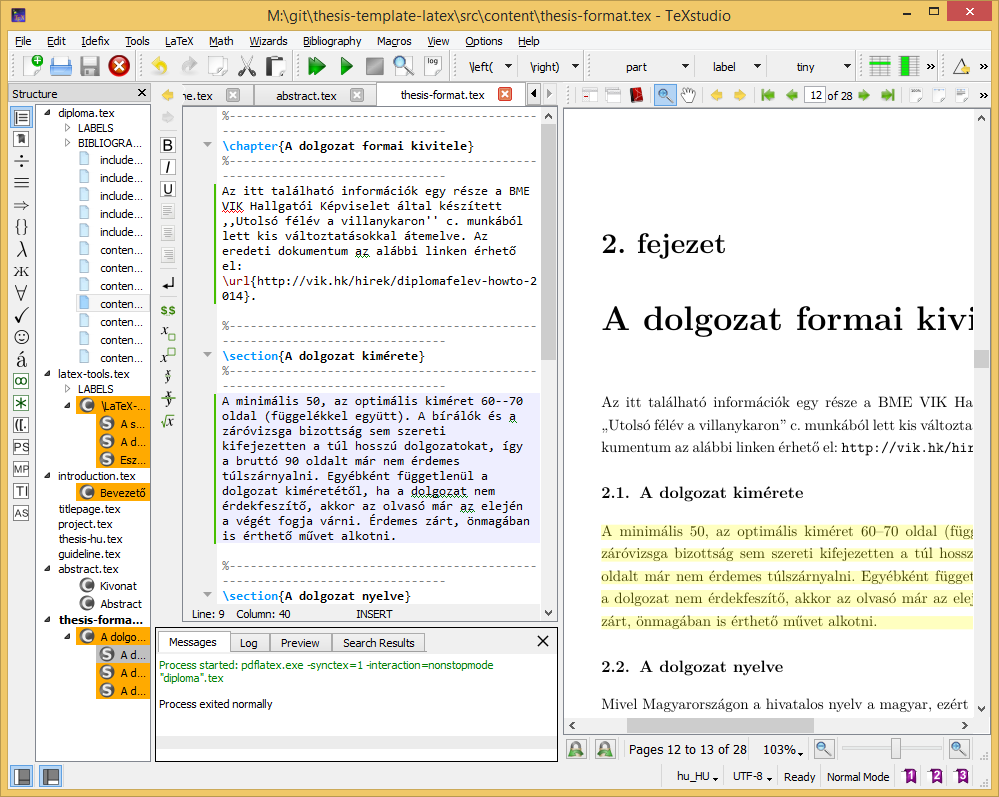
\includegraphics[width=150mm, keepaspectratio]{figures/TeXstudio.png}
\caption{A TeXstudio \LaTeX-szerkesztő.}
\label{fig:TeXstudio}
\end{figure}

A TeXstudio telepítése után érdemes még letölteni a magyar nyelvű helyesírásellenőrző-szótárakat hozzá. A TeXstudio az OpenOffice-hoz használatos formátumot tudja kezelni. A TeXstudio beállításainál a \verb+General+ fülön a \verb+Dictionaries+ résznél tudjuk megadni, hogy melyik szótárat használja.

Egy másik használható Windows alapú szerkesztőprogram a LEd\footnote{A LEd hivatalos oldala: \url{http://www.latexeditor.org/}} (LaTeX Editor), a TeXstudio azonban stabilabb, gyorsabb, és jobban használható.

%----------------------------------------------------------------------------
\section{A dokumentum lefordítása Windows alatt}
%----------------------------------------------------------------------------
A TeXstudio és a LEd kizárólag szerkesztőprogram (bár az utóbbiban DVI-nézegető is van), így a dokumentum fordításához szükséges eszközöket nem tartalmazza. Windows alatt alapvetően két lehetőség közül érdemes választani: MiKTeX (\url{http://miktex.org/}) és TeX Live (\url{http://www.tug.org/texlive/}) programcsomag. Az utóbbi működik Mac OS X, GNU/Linux alatt és Unix-származékokon is. A MiKTeX egy alapcsomag telepítése után mindig letölti a használt funkciókhoz szükséges, de lokálisan hiányzó \TeX-csomagokat, míg a TeX Live DVD ISO verzóban férhető hozzá. Ez a dokumentum TeX Live 2008 programcsomag segítségével fordult, amelynek DVD ISO verziója a megadott oldalról letölthető. A sablon lefordításához a disztribúcióban szereplő \verb+magyar.ldf+ fájlt a \verb+http://www.math.bme.hu/latex/+ változatra kell cserélni, vagy az utóbbi változatot be kell másolni a projekt-könyvtárba (ahogy ezt meg is tettük a sablonban) különben anomáliák tapasztalhatók a dokumentumban (pl. az ábra- és táblázat-aláírások formátuma nem a beállított lesz, vagy bizonyos oldalakon megjelenik alapértelmezésben egy fejléc). A TeX Live 2008-at még nem kell külön telepíteni a gépre, elegendő DVD-ről (vagy az ISO fájlból közvetlenül, pl. DaemonTools-szal) használni.

Ha a MiKTeX csomagot használjuk, akkor parancssorból a következő módon tudjuk újrafordítani a teljes dokumentumot:

\begin{lstlisting}[language=bash,frame=single,float=!ht]
$ texify -p thesis.tex
\end{lstlisting}

A \verb+texify+ parancs a MiKTex programcsomag \verb+miktex/bin+ alkönyvtárában található. A parancs gondoskodik arról, hogy a szükséges lépéseket (fordítás, hivatkozások generálása stb.) a megfelelő sorrendben elvégezze. A \verb+-p+ kapcsoló hatására PDF-et generál. A fordítást és az ideiglenes fájlok törlését elvégezhetjük a sablonhoz mellékelt \verb+manual_build.bat+ szkript segítségével is.

A \TeX-eszközöket tartalmazó programcsomag binárisainak elérési útját gyakran be kell állítani a szerkesztőprogramban, például TeXstudio esetén legegyszerűbben az \verb+Options / Configure TeXstudio... / Commands+ menüponttal előhívott dialógusablakban tehetjük ezt meg.

A PDF-\LaTeX~használata esetén a generált dokumentum közvetlenül PDF-formátumban áll rendelkezésre. Amennyiben a PDF-fájl egy PDF-nézőben (pl. Adobe Acrobat Reader vagy Foxit PDF Reader) meg van nyitva, akkor a fájlleírót a PDF-néző program tipikusan lefoglalja. Ilyen esetben a dokumentum újrafordítása hibaüzenettel kilép. Ha bezárjuk és újra megnyitjuk a PDF dokumentumot, akkor pedig a PDF-nézők többsége az első oldalon nyitja meg a dokumentumot, nem a legutóbb olvasott oldalon. Ezzel szemben például az egyszerű és ingyenes \textcolor{blue}{Sumatra PDF} nevű program képes arra, hogy a megnyitott dokumentum megváltozását detektálja, és frissítse a nézetet az aktuális oldal megtartásával.

%----------------------------------------------------------------------------
\section{Eszközök Linuxhoz}
%----------------------------------------------------------------------------
Linux operációs rendszer alatt is rengeteg szerkesztőprogram van, pl. a KDE alapú Kile jól használható. Ez ingyenesen letölthető, vagy éppenséggel az adott Linux-disztribúció eleve tartalmazza, ahogyan a dokumentum fordításához szükséges csomagokat is. Az Ubuntu Linux disztribúciók alatt például legtöbbször a \verb+texlive-*+ csomagok telepítésével használhatók a \LaTeX-eszközök. A jelen sablon fordításához szükséges csomagok (kb. 0,5 GB) az alábbi paranccsal telepíthetők:

\begin{lstlisting}[language=bash,morekeywords={sudo,apt\-get},alsoletter={-},breaklines=true]
$ sudo apt-get install texlive-latex-extra texlive-fonts-extra texlive-fonts-recommended texlive-xetex texlive-science
\end{lstlisting}

Amennyiben egy újabb csomag hozzáadása után hiányzó fájlra utaló hibát kapunk a fordítótól, telepítenünk kell az azt tartalmazó TeX Live csomagot. Ha pl. a \verb+bibentry+ csomagot szeretnénk használni, futtassuk az alábbi parancsot:

\begin{lstlisting}[language=bash,morekeywords={apt\-cache},alsoletter={-},breaklines=true]
$ apt-cache search bibentry
texlive-luatex - TeX Live: LuaTeX packages
\end{lstlisting}

Majd telepítsük fel a megfelelő TeX Live csomagot, jelen esetben a `texlive-lualatex`-et. (Egy LaTeX csomag több TeX Live csomagban is szerepelhet.)

Ha gyakran szerkesztünk más \LaTeX dokumentumokat is, kényelmes és biztos megoldás a teljes TeX Live disztribúció telepítése, ez azonban kb. 4 GB helyet igényel.

\begin{lstlisting}[language=bash,morekeywords={sudo,apt\-get},alsoletter={-},breaklines=true]
sudo apt-get install texlive-full
\end{lstlisting}

%%----------------------------------------------------------------------------
\chapter{A dolgozat formai kivitele}
%----------------------------------------------------------------------------
Az itt található információk egy része a BME VIK Hallgatói Képviselet által készített ,,Utolsó félév a villanykaron'' c. munkából lett kis változtatásokkal átemelve. Az eredeti dokumentum az alábbi linken érhető el: \url{http://vik.hk/hirek/diplomafelev-howto-2015}.

%----------------------------------------------------------------------------
\section{A dolgozat kimérete}
%----------------------------------------------------------------------------
Szakdolgozat esetében minimum 30, 45 körüli ajánlott oldalszám lehet az iránymutató. De mindenképp érdemes rákérdezni a konzulensnél is az elvárásokra, mert tanszékenként változóak lehetnek az elvárások.

Mesterképzésen a Diplomatervezés 1 esetében a beszámoló még inkább az Önálló laboratóriumi beszámolókhoz hasonlít, tanszékenként eltérő formai követelményekkel, -- egy legalább 30 oldal körüli dolgozat az elvárt -- és az elmúlt fél éves munkáról szól. De egyben célszerű, ha ez a végleges diplomaterv alapja is. (A végleges 60-90 oldal körülbelül a hasznos részre nézve)


%----------------------------------------------------------------------------
\section{A dolgozat nyelve}
%----------------------------------------------------------------------------
Mivel Magyarországon a hivatalos nyelv a magyar, ezért alapértelmezésben magyarul kell megírni a dolgozatot. Aki külföldi posztgraduális képzésben akar részt venni, nemzetközi szintű tudományos kutatást szeretne végezni, vagy multinacionális cégnél akar elhelyezkedni, annak célszerű angolul megírnia diplomadolgozatát. Mielőtt a hallgató az angol nyelvű verzió mellett dönt, erősen ajánlott mérlegelni, hogy ez mennyi többletmunkát fog a hallgatónak jelenteni fogalmazás és nyelvhelyesség terén, valamint -- nem utolsó sorban -- hogy ez mennyi többletmunkát fog jelenteni a konzulens illetve bíráló számára. Egy nehezen olvasható, netalán érthetetlen szöveg teher minden játékos számára.

%----------------------------------------------------------------------------
\section{A dokumentum nyomdatechnikai kivitele}
%----------------------------------------------------------------------------
A dolgozatot A4-es fehér lapra nyomtatva, 2,5 centiméteres margóval (+1~cm kötésbeni), 11--12 pontos betűmérettel, talpas betűtípussal és másfeles sorközzel célszerű elkészíteni.

Annak érdekében, hogy a dolgozat külsőleg is igényes munka benyomását keltse, érdemes figyelni az alapvető tipográfiai szabályok betartására~\cite{Jeney}.

%% !TeX spellcheck = hu_HU
% !TeX encoding = UTF-8
% !TeX program = xelatex
%----------------------------------------------------------------------------
\chapter{A \LaTeX-sablon használata}
%----------------------------------------------------------------------------

Ebben a fejezetben röviden, implicit módon bemutatjuk a sablon használatának módját, ami azt jelenti, hogy sablon használata ennek a dokumentumnak a forráskódját tanulmányozva válik teljesen világossá. Amennyiben a szoftver-keretrendszer telepítve van, a sablon alkalmazása és a dolgozat szerkesztése \LaTeX-ben a sablon segítségével tapasztalataink szerint jóval hatékonyabb, mint egy WYSWYG (\emph{What You See is What You Get}) típusú szövegszerkesztő esetén (pl. Microsoft Word, OpenOffice).

%----------------------------------------------------------------------------
\section{Címkék és hivatkozások}
%----------------------------------------------------------------------------
A \LaTeX~dokumentumban címkéket (\verb+\label+) rendelhetünk ábrákhoz, táblázatokhoz, fejezetekhez, listákhoz, képletekhez stb. Ezekre a dokumentum bármely részében hivatkozhatunk, a hivatkozások automatikusan feloldásra kerülnek.

A sablonban makrókat definiáltunk a hivatkozások megkönnyítéséhez. Ennek megfelelően minden ábra (\emph{figure}) címkéje \verb+fig:+ kulcsszóval kezdődik, míg minden táblázat (\emph{table}), képlet (\emph{equation}), fejezet (\emph{section}) és lista (\emph{listing}) rendre a \verb+tab:+, \verb+eq:+, \verb+sec:+ és \verb+lst:+ kulcsszóval kezdődik, és a kulcsszavak után tetszőlegesen választott címke használható. Ha ezt a konvenciót betartjuk, akkor az előbbi objektumok számára rendre a \verb+\figref+, \verb+\tabref+, \verb+\eqref+, \verb+\sectref+ és \verb+\listref+ makrókkal hivatkozhatunk. A makrók paramétere a címke, amelyre hivatkozunk (a kulcsszó nélkül). Az összes említett hivatkozástípus, beleértve az \verb+\url+ kulcsszóval bevezetett web-hivatkozásokat is a  \verb+hyperref+\footnote{Segítségével a dokumentumban megjelenő hivatkozások nem csak dinamikussá válnak, de színezhetők is, bővebbet erről a csomag dokumentációjában találunk. Ez egyúttal egy példa lábjegyzet írására.} csomagnak köszönhetően aktívak a legtöbb PDF-nézegetőben, rájuk kattintva a dokumentum megfelelő oldalára ugrik a PDF-néző vagy a megfelelő linket megnyitja az alapértelmezett böngészővel. A \verb+hyperref+ csomag a kimeneti PDF-dokumentumba könyvjelzőket is készít a tartalomjegyzékből. Ez egy szintén aktív tartalomjegyzék, amelynek elemeire kattintva a nézegető behozza a kiválasztott fejezetet.

%----------------------------------------------------------------------------
\section{Ábrák és táblázatok}
%----------------------------------------------------------------------------
Használjunk vektorgrafikus ábrákat, ha van rá módunk. PDFLaTeX használata esetén PDF formátumú ábrákat lehet beilleszteni könnyen, az EPS (PostScript) vektorgrafikus képformátum beillesztését a PDFLaTeX közvetlenül nem támogatja (de lehet konvertálni, lásd később). Ha vektorgrafikus formában nem áll rendelkezésünkre az ábra, akkor a  veszteségmentes PNG, valamint a veszteséges JPEG formátumban érdemes elmenteni.  Figyeljünk arra, hogy ilyenkor a képek felbontása elég nagy legyen ahhoz, hogy nyomtatásban is megfelelő minőséget nyújtson (legalább 300 dpi javasolt). A dokumentumban felhasznált képfájlokat a dokumentum forrása mellett érdemes tartani, archiválni, mivel ezek hiányában a dokumentum nem fordul újra. Ha lehet, a vektorgrafikus képeket vektorgrafikus formátumban is érdemes elmenteni az újrafelhasználhatóság (az átszerkeszthetőség) érdekében.

Kapcsolási rajzok legtöbbször kimásolhatók egy vektorgrafikus programba (pl. CorelDraw) és onnan nagyobb felbontással raszterizálva kimenthatők PNG formátumban. Ugyanakkor kiváló ábrák készíthetők Microsoft Visio vagy hasonló program használatával is: Visio-ból az ábrák közvetlenül PDF-be is menthetők.

Lehetőségeink Matlab ábrák esetén:
\begin{itemize}
	\item Képernyőlopás (\emph{screenshot}) is elfogadható minőségű lehet a dokumentumban, de általában jobb felbontást is el lehet érni más módszerrel.
	\item A Matlab ábrát a \verb+File/Save As+ opcióval lementhetjük PNG formátumban (ugyanaz itt is érvényes, mint korábban, ezért nem javasoljuk).
	\item A Matlab ábrát az \verb+Edit/Copy figure+ opcióval kimásolhatjuk egy vektorgrafikus programba is és onnan nagyobb felbontással raszterizálva kimenthatjük PNG formátumban (nem javasolt).
	\item Javasolt megoldás: az ábrát a \verb+File/Save As+ opcióval EPS \emph{vektorgrafikus} formátumban elmentjük, PDF-be konvertálva beillesztjük a dolgozatba.
\end{itemize}
Az EPS kép az \verb+epstopdf+ programmal\footnote{a korábban említett \LaTeX-disztribúciókban megtalálható} konvertálható PDF formátumba. Célszerű egy batch-fájlt készíteni az összes EPS ábra lefordítására az alábbi módon (ez Windows alatt működik).
\begin{lstlisting}[language=]
@echo off
for %%j in (*.eps) do (
  echo converting file "%%j"
  epstopdf "%%j"
)
echo done .
\end{lstlisting}

Egy ilyen parancsfájlt (\verb+convert.cmd+) elhelyeztük a sablon \verb+figures\eps+ könyvtárába, így a felhasználónak csak annyi a dolga, hogy a \verb+figures\eps+ könyvtárba kimenti az EPS formátumú vektorgrafikus képet, majd lefuttatja a \verb+convert.cmd+ parancsfájlt, ami PDF-be konvertálja az EPS fájlt.

Ezek után a PDF-ábrát ugyanúgy lehet a dokumentumba beilleszteni, mint a PNG-t vagy a JPEG-et. A megoldás előnye, hogy a lefordított dokumentumban is vektorgrafikusan tárolódik az ábra, így a mérete jóval kisebb, mintha raszterizáltuk volna beillesztés előtt. Ez a módszer minden -- az EPS formátumot ismerő -- vektorgrafikus program (pl. CorelDraw) esetén is használható.

A képek beillesztésére \az+\refstruc{sec:LatexTools}ben mutattunk be példát (\refstruc{fig:TeXstudio}). Az előző mondatban egyúttal az automatikusan feloldódó ábrahivatkozásra is láthatunk példát. Több képfájlt is beilleszthetünk egyetlen ábrába. Az egyes képek közötti horizontális és vertikális margót metrikusan szabályozhatjuk (\refstruc{fig:HVSpaces}). Az ábrák elhelyezését számtalan tipográfiai szabály egyidejű teljesítésével a fordító maga végzi, a dokumentum írója csak preferenciáit jelezheti a fordító felé (olykor ez bosszúságot is okozhat, ilyenkor pl. a kép méretével lehet játszani).

\begin{figure}[!ht]
	\centering
	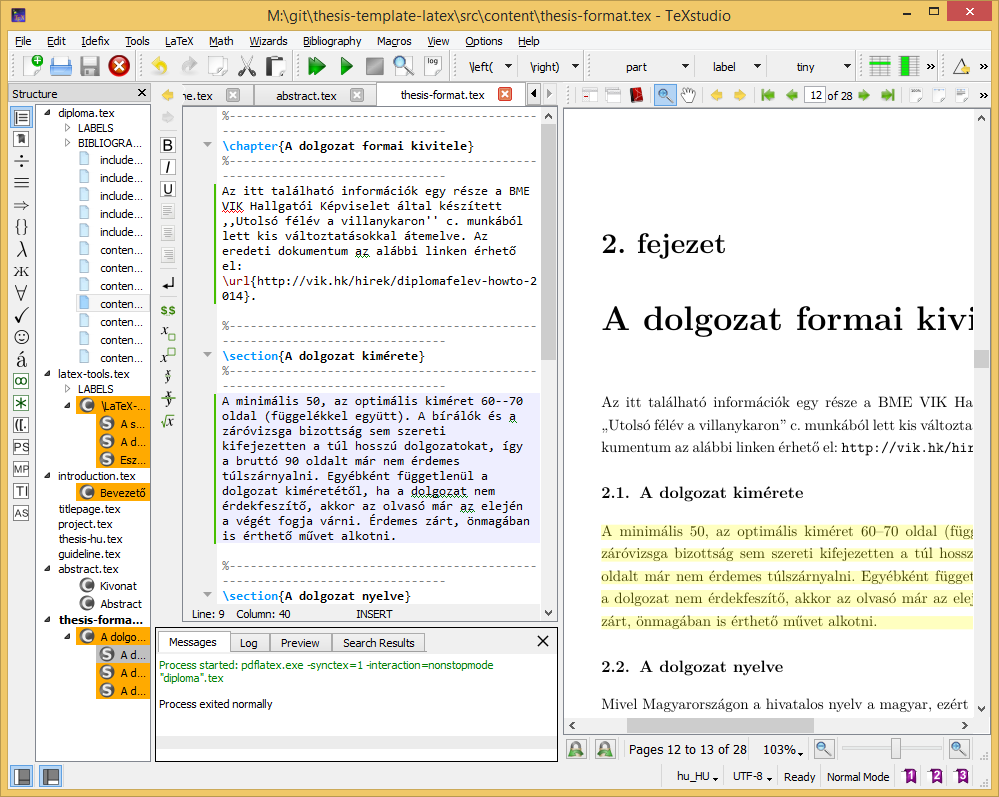
\includegraphics[width=67mm, keepaspectratio]{figures/TeXstudio.png}\hspace{1cm}
	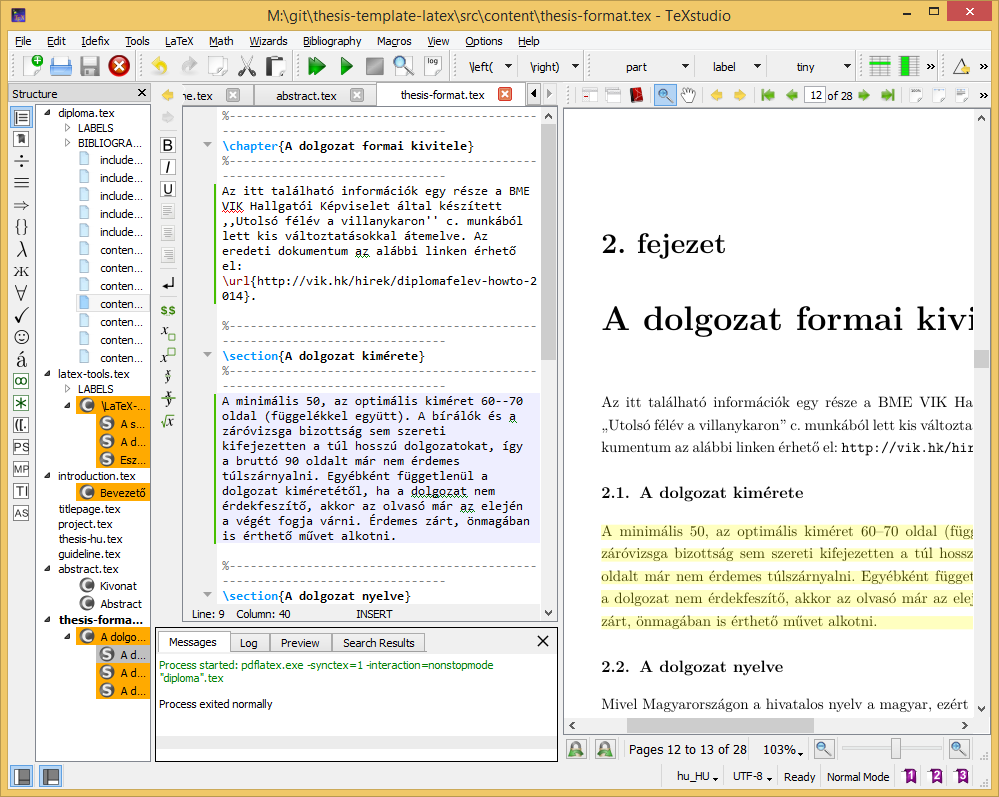
\includegraphics[width=67mm, keepaspectratio]{figures/TeXstudio.png}\\\vspace{5mm}
	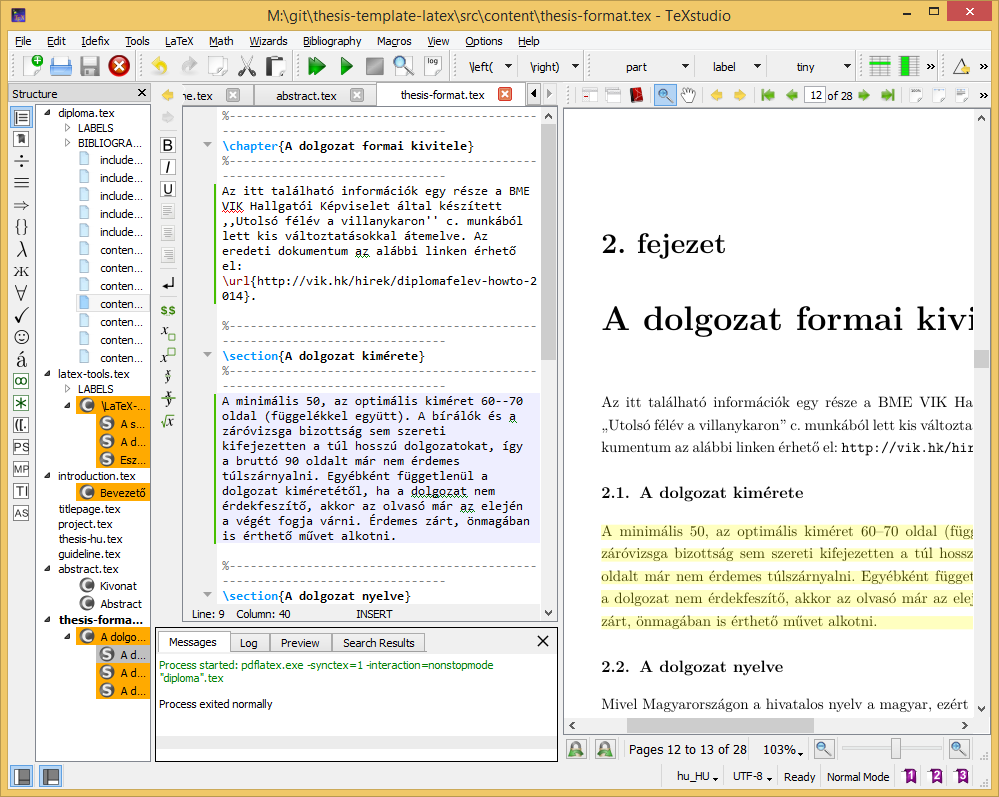
\includegraphics[width=67mm, keepaspectratio]{figures/TeXstudio.png}\hspace{1cm}
	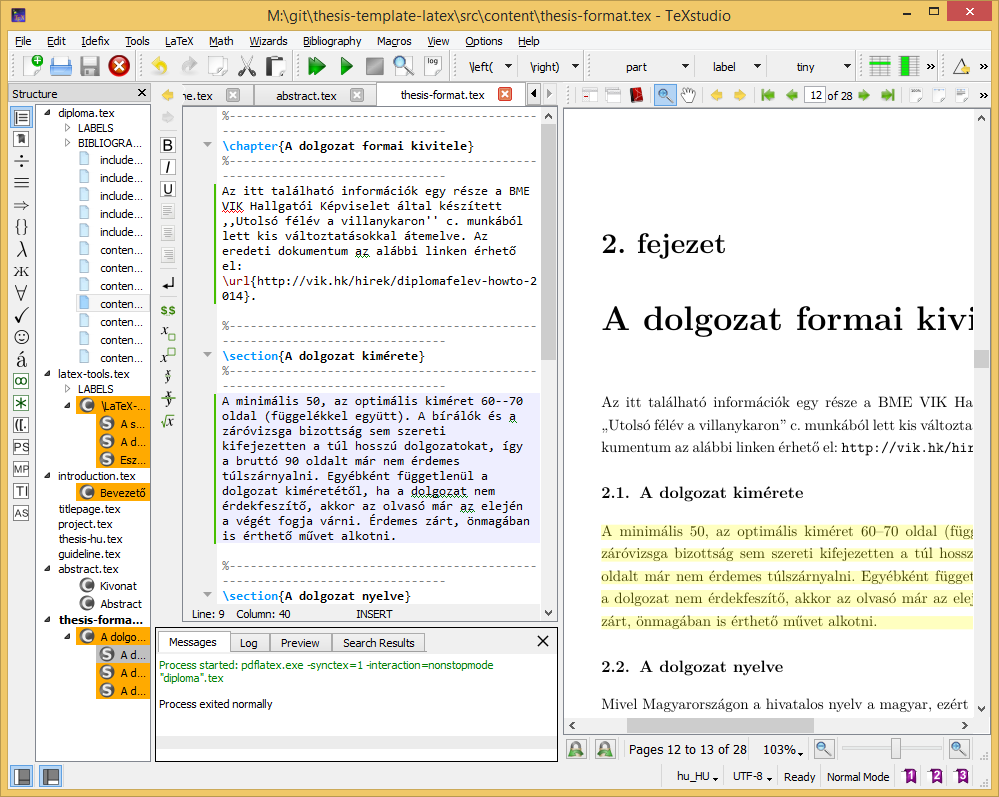
\includegraphics[width=67mm, keepaspectratio]{figures/TeXstudio.png}
	\caption{Több képfájl beillesztése esetén térközöket is érdemes használni.}
	\label{fig:HVSpaces}
\end{figure}

A táblázatok használatára \aref{tab:TabularExample}~táblázat mutat példát. A táblázatok formázásához hasznos tanácsokat találunk a \verb+booktabs+ csomag dokumentációjában.

\begin{table}[ht]
	\footnotesize
	\centering
	\begin{tabular}{ l c c }
		\toprule
		Órajel & Frekvencia & Cél pin \\
		\midrule
		CLKA & 100 MHz & FPGA CLK0\\
		CLKB & 48 MHz  & FPGA CLK1\\
		CLKC & 20 MHz  & Processzor\\
		CLKD & 25 MHz  & Ethernet chip \\
		CLKE & 72 MHz  & FPGA CLK2\\
		XBUF & 20 MHz  & FPGA CLK3\\
		\bottomrule
	\end{tabular}
	\caption{Az órajel-generátor chip órajel-kimenetei.}
	\label{tab:TabularExample}
\end{table}


%----------------------------------------------------------------------------
\section{Felsorolások és listák}
%----------------------------------------------------------------------------
Számozatlan felsorolásra mutat példát a jelenlegi bekezdés:
\begin{itemize}
	\item \emph{első bajusz:} ide lehetne írni az első elem kifejését,
	\item \emph{második bajusz:} ide lehetne írni a második elem kifejését,
	\item \emph{ez meg egy szakáll:} ide lehetne írni a harmadik elem kifejését.
\end{itemize}

Számozott felsorolást is készíthetünk az alábbi módon:
\begin{enumerate}
	\item \emph{első bajusz:} ide lehetne írni az első elem kifejését, és ez a kifejtés így néz ki, ha több sorosra sikeredik,
	\item \emph{második bajusz:} ide lehetne írni a második elem kifejését,
	\item \emph{ez meg egy szakáll:} ide lehetne írni a harmadik elem kifejését.
\end{enumerate}
A felsorolásokban sorok végén vessző, az utolsó sor végén pedig pont a szokásos írásjel. Ez alól kivételt képezhet, ha az egyes elemek több teljes mondatot tartalmaznak.

Listákban a dolgozat szövegétől elkülönítendő kódrészleteket, programsorokat, pszeudo-kódokat jeleníthetünk meg (\ref{lst:Example}.~kódrészlet).
\begin{lstlisting}[language=tex,caption=A fenti számozott felsorolás \LaTeX-forráskódja,label=lst:Example]
\begin{enumerate}
	\item \emph{els(*@ő@*) bajusz:} ide lehetne írni az els(*@ő@*) elem kifejését,
	és ez a kifejtés így néz ki, ha több sorosra sikeredik,
	\item \emph{második bajusz:} ide lehetne írni a második elem kifejését,
	\item \emph{ez meg egy szakáll:} ide lehetne írni a harmadik elem kifejését.
\end{enumerate}
\end{lstlisting}
A lista keretét, háttérszínét, egész stílusát megválaszthatjuk. Ráadásul különféle programnyelveket és a nyelveken belül kulcsszavakat is definiálhatunk, ha szükséges. Erről bővebbet a \verb+listings+ csomag hivatalos leírásában találhatunk.

%----------------------------------------------------------------------------
\section{Képletek}
%----------------------------------------------------------------------------
Ha egy formula nem túlságosan hosszú, és nem akarjuk hivatkozni a szövegből, mint például a $e^{i\pi}+1=0$ képlet, \emph{szövegközi képletként} szokás leírni. Csak, hogy másik példát is lássunk, az $U_i=-d\Phi/dt$ Faraday-törvény a $\rot E=-\frac{dB}{dt}$ differenciális alakban adott Maxwell-egyenlet felületre vett integráljából vezethető le. Látható, hogy a \LaTeX-fordító a sorközöket betartja, így a szöveg szedése esztétikus marad szövegközi képletek használata esetén is.

Képletek esetén az általános konvenció, hogy a kisbetűk skalárt, a kis félkövér betűk ($\mathbf{v}$) oszlopvektort -- és ennek megfelelően $\mathbf{v}^T$ sorvektort -- a kapitális félkövér betűk ($\mathbf{V}$) mátrixot jelölnek. Ha ettől el szeretnénk térni, akkor az alkalmazni kívánt jelölésmódot célszerű külön alfejezetben definiálni. Ennek megfelelően, amennyiben $\mathbf{y}$ jelöli a mérések vektorát, $\mathbf{\vartheta}$ a paraméterek vektorát és $\hat{\mathbf{y}}=\mathbf{X}\vartheta$ a paraméterekben lineáris modellt, akkor a \emph{Least-Squares} értelemben optimális paraméterbecslő $\hat{\mathbf{\vartheta}}_{LS}=(\mathbf{X}^T\mathbf{X})^{-1}\mathbf{X}^T\mathbf{y}$ lesz.

Emellett kiemelt, sorszámozott képleteket is megadhatunk, ennél az \verb+equation+ és a \verb+eqnarray+ környezetek helyett a korszerűbb \verb+align+ környezet alkalmazását javasoljuk (több okból, különféle problémák elkerülése végett, amelyekre most nem térünk ki). Tehát
\begin{align}
\dot{\mathbf{x}}&=\mathbf{A}\mathbf{x}+\mathbf{B}\mathbf{u},\\
\mathbf{y}&=\mathbf{C}\mathbf{x},
\end{align}
ahol $\mathbf{x}$ az állapotvektor, $\mathbf{y}$ a mérések vektora és $\mathbf{A}$, $\mathbf{B}$ és $\mathbf{C}$ a rendszert leíró paramétermátrixok. Figyeljük meg, hogy a két egyenletben az egyenlőségjelek egymáshoz igazítva jelennek meg, mivel a mindkettőt az \& karakter előzi meg a kódban. Lehetőség van számozatlan kiemelt képlet használatára is, például
\begin{align}
\dot{\mathbf{x}}&=\mathbf{A}\mathbf{x}+\mathbf{B}\mathbf{u},\nonumber\\
\mathbf{y}&=\mathbf{C}\mathbf{x}\nonumber.
\end{align}
Mátrixok felírására az $\mathbf{A}\mathbf{x}=\mathbf{b}$ inhomogén lineáris egyenlet részletes kifejtésével mutatunk példát:
\begin{align}
\begin{bmatrix}
a_{11} & a_{12} & \dots & a_{1n}\\
a_{21} & a_{22} & \dots & a_{2n}\\
\vdots & \vdots & \ddots & \vdots\\
a_{m1} & a_{m2} & \dots & a_{mn}
\end{bmatrix}
\begin{pmatrix}x_1\\x_2\\\vdots\\x_n\end{pmatrix}=
\begin{pmatrix}b_1\\b_2\\\vdots\\b_m\end{pmatrix}.
\end{align}
A \verb+\frac+ utasítás hatékonyságát egy általános másodfokú tag átviteli függvényén keresztül mutatjuk be, azaz
\begin{align}
W(s)=\frac{A}{1+2T\xi s+s^2T^2}.
\end{align}
A matematikai mód minden szimbólumának és képességének a bemutatására természetesen itt nincs lehetőség, de gyors referenciaként hatékonyan használhatók a következő linkek:\\
\indent\url{http://www.artofproblemsolving.com/LaTeX/AoPS_L_GuideSym.php},\\
\indent\url{http://www.ctan.org/tex-archive/info/symbols/comprehensive/symbols-a4.pdf},\\
\indent\url{ftp://ftp.ams.org/pub/tex/doc/amsmath/short-math-guide.pdf}.\\
Ez pedig itt egy magyarázat, hogy miért érdemes \verb+align+ környezetet használni:\\
\indent\url{http://texblog.net/latex-archive/maths/eqnarray-align-environment/}.

%----------------------------------------------------------------------------
\section{Irodalmi hivatkozások}
\label{sec:HowtoReference}
%----------------------------------------------------------------------------
Egy \LaTeX~dokumentumban az irodalmi hivatkozások definíciójának két módja van. Az egyik a \verb+\thebibliograhy+ környezet használata a dokumentum végén, az \verb+\end{document}+ lezárás előtt.
\begin{lstlisting}[language=tex]
\begin{thebibliography}{9}

\bibitem{Lamport94} Leslie Lamport, \emph{\LaTeX: A Document Preparation System}.
Addison Wesley, Massachusetts, 2nd Edition, 1994.

\end{thebibliography}
\end{lstlisting}

Ezek után a dokumentumban a \verb+\cite{Lamport94}+ utasítással hivatkozhatunk a forrásra. A fenti megadás viszonylag kötetlen, a szerző maga formázza az irodalomjegyzéket (ami gyakran inkonzisztens eredményhez vezet).

Egy sokkal professzionálisabb módszer a BiB\TeX{} használata, ezért ez a sablon is ezt támogatja. Ebben az esetben egy külön szöveges adatbázisban definiáljuk a forrásmunkákat, és egy külön stílusfájl határozza meg az irodalomjegyzék kinézetét. Ez, összhangban azzal, hogy külön formátumkonvenció határozza meg a folyóirat-, a könyv-, a konferenciacikk- stb. hivatkozások kinézetét az irodalomjegyzékben (a sablon használata esetén ezzel nem is kell foglalkoznia a hallgatónak, de az eredményt célszerű ellenőrizni). felhasznált hivatkozások adatbázisa egy \verb+.bib+ kiterjesztésű szöveges fájl, amelynek szerkezetét a \Aref{lst:Bibtex} kódrészlet demonstrálja. A forrásmunkák bevitelekor a sor végi vesszők külön figyelmet igényelnek, mert hiányuk a BiB\TeX-fordító hibaüzenetét eredményezi. A forrásmunkákat típus szerinti kulcsszó vezeti be (\verb+@book+ könyv, \verb+@inproceedings+ konferenciakiadványban megjelent cikk, \verb+@article+ folyóiratban megjelent cikk, \verb+@techreport+ valamelyik egyetem gondozásában megjelent műszaki tanulmány, \verb+@manual+ műszaki dokumentáció esetén stb.). Nemcsak a megjelenés stílusa, de a kötelezően megadandó mezők is típusról-típusra változnak. Egy jól használható referencia a \url{http://en.wikipedia.org/wiki/BibTeX} oldalon található.

\begin{lstlisting}[caption=Példa szöveges irodalomjegyzék-adatbázisra Bib\TeX{} használata esetén.,label=lst:Bibtex]
@book{Wettl04,
  author    = {Ferenc Wettl and Gyula Mayer and Péter Szabó},
  publisher = {Panem Könyvkiadó},
  title     = {\LaTeX~kézikönyv},
  year      = {2004},
}

@article{Candy86,
  author       = {James C. Candy},
  journaltitle = {{IEEE} Trans.\ on Communications},
  month        = {01},
  note         = {\doi{10.1109/TCOM.1986.1096432}},
  number       = {1},
  pages        = {72--76},
  title        = {Decimation for Sigma Delta Modulation},
  volume       = {34},
  year         = {1986},
}

@inproceedings{Lee87,
  author    = {Wai L. Lee and Charles G. Sodini},
  booktitle = {Proc.\ of the IEEE International Symposium on Circuits and Systems},
  location  = {Philadelphia, PA, USA},
  month     = {05~4--7},
  pages     = {459--462},
  title     = {A Topology for Higher Order Interpolative Coders},
  vol       = {2},
  year      = {1987},
}

@thesis{KissPhD,
  author      = {Peter Kiss},
  institution = {Technical University of Timi\c{s}oara, Romania},
  month       = {04},
  title       = {Adaptive Digital Compensation of Analog Circuit Imperfections for Cascaded Delta-Sigma Analog-to-Digital Converters},
  type        = {phdthesis},
  year        = {2000},
}

@manual{Schreier00,
  author       = {Richard Schreier},
  month        = {01},
  note         = {\url{http://www.mathworks.com/matlabcentral/fileexchange/}},
  organization = {Oregon State University},
  title        = {The Delta-Sigma Toolbox v5.2},
  year         = {2000},
}

@misc{DipPortal,
  author       = {{Budapesti Műszaki és Gazdaságtudományi Egyetem Villamosmérnöki és Informatikai Kar}},
  howpublished = {\url{http://diplomaterv.vik.bme.hu/}},
  title        = {Diplomaterv portál (2011. február 26.)},
}

@incollection{Mkrtychev:1997,
  author    = {Mkrtychev, Alexey},
  booktitle = {Logical Foundations of Computer Science},
  doi       = {10.1007/3-540-63045-7_27},
  editor    = {Adian, Sergei and Nerode, Anil},
  isbn      = {978-3-540-63045-6},
  pages     = {266-275},
  publisher = {Springer Berlin Heidelberg},
  series    = {Lecture Notes in Computer Science},
  title     = {Models for the logic of proofs},
  url       = {http://dx.doi.org/10.1007/3-540-63045-7_27},
  volume    = {1234},
  year      = {1997},
}
\end{lstlisting}

A stílusfájl egy \verb+.sty+ kiterjesztésű fájl, de ezzel lényegében nem kell foglalkozni, mert vannak beépített stílusok, amelyek jól használhatók. Ez a sablon a BiB\TeX-et használja, a hozzá tartozó adatbázisfájl a \verb+mybib.bib+ fájl. Megfigyelhető, hogy az irodalomjegyzéket a dokumentum végére (a \verb+\end{document}+ utasítás elé) beillesztett \verb+\bibliography{mybib}+ utasítással hozhatjuk létre, a stílusát pedig ugyanitt a  \verb+\bibliographystyle{plain}+ utasítással adhatjuk meg. Ebben az esetben a \verb+plain+ előre definiált stílust használjuk (a sablonban is ezt állítottuk be). A \verb+plain+ stíluson kívül természetesen számtalan más előre definiált stílus is létezik. Mivel a \verb+.bib+ adatbázisban ezeket megadtuk, a BiB\TeX-fordító is meg tudja különböztetni a szerzőt a címtől és a kiadótól, és ez alapján automatikusan generálódik az irodalomjegyzék a stílusfájl által meghatározott stílusban.

Az egyes forrásmunkákra a szövegből továbbra is a \verb+\cite+ paranccsal tudunk hivatkozni, így \aref{lst:Bibtex}.~kódrészlet esetén a hivatkozások rendre \verb+\cite{Wettl04}+, \verb+\cite{Candy86}+, \verb+\cite{Lee87}+, \verb+\cite{KissPhD}+, \verb+\cite{Schreirer00}+,
\verb+\cite{Mkrtychev:1997}+ és \verb+\cite{DipPortal}+. Az egyes forrásmunkák sorszáma az irodalomjegyzék bővítésekor változhat. Amennyiben az aktuális számhoz illeszkedő névelőt szeretnénk használni, használjuk az \verb+\acite{}+ parancsot.

Az irodalomjegyzékben alapértelmezésben csak azok a forrásmunkák jelennek meg, amelyekre található hivatkozás a szövegben, és ez így alapvetően helyes is, hiszen olyan forrásmunkákat nem illik az irodalomjegyzékbe írni, amelyekre nincs hivatkozás.

Mivel a fordítási folyamat során több lépésben oldódnak fel a szimbólumok, ezért gyakran többször is le kell fordítani a dokumentumot. Ilyenkor ez első 1-2 fordítás esetleg szimbólum-feloldásra vonatkozó figyelmeztető üzenettel zárul. Ha hibaüzenettel zárul bármelyik fordítás, akkor nincs értelme megismételni, hanem a hibát kell megkeresni. A \verb+.bib+ fájl megváltoztatáskor sokszor nincs hatása a változtatásnak azonnal, mivel nem mindig fut újra a BibTeX fordító. Ezért célszerű a változtatás után azt manuálisan is lefuttatni (TeXstudio esetén \verb+Tools/Bibliography+).

Hogy a szövegbe ágyazott hivatkozások kinézetét demonstráljuk, itt most sorban meghivatkozzuk a \cite{Wettl04}, \cite{Candy86}, \cite{Lee87}, \cite{KissPhD}, \cite{Schreier00} és \acite{Mkrtychev:1997}\footnote{Informatikai témában gyakran hivatkozunk cikkeket a Springer LNCS valamely kötetéből, ez a hivatkozás erre mutat egy helyes példát.} forrásmunkát, valamint \acite{DipPortal} weboldalt.

Megjegyzendő, hogy az ékezetes magyar betűket is tartalmazó \verb+.bib+ fájl az \verb+inputenc+ csomaggal betöltött \verb+latin2+ betűkészlet miatt fordítható. Ugyanez a \verb+.bib+ fájl hibaüzenettel fordul egy olyan dokumentumban, ami nem tartalmazza a \verb+\usepackage[latin2]{inputenc}+ sort. Speciális igény esetén az irodalmi adatbázis általánosabb érvényűvé tehető, ha az ékezetes betűket speciális latex karakterekkel helyettesítjük a \verb+.bib+ fájlban, pl. á helyett \verb+\'{a}+-t vagy ő helyett \verb+\H{o}+-t írunk.

Irodalomhivatkozásokat célszerű először olyan szolgáltatásokban keresni, ahol jó minőségű bejegyzések találhatók (pl. ACM Digital Library,\footnote{\url{https://dl.acm.org/}} DBLP,\footnote{\url{http://dblp.uni-trier.de/}} IEEE Xplore,\footnote{\url{http://ieeexplore.ieee.org/}} SpringerLink\footnote{\url{https://link.springer.com/}}) és csak ezek után használni kevésbé válogatott forrásokat (pl. Google Scholar\footnote{\url{http://scholar.google.com/}}). A jó minőségű bejegyzéseket is érdemes megfelelően tisztítani.\footnote{\url{https://github.com/FTSRG/cheat-sheets/wiki/BibTeX-Fixing-entries-from-common-sources}} A sablon angol nyelvű változatában használt \texttt{plainnat} beállítás egyik sajátossága, hogy a cikkhez generált hivatkozás a cikk DOI-ját és URL-jét is tartalmazza, ami gyakran duplikátumhoz vezet -- érdemes tehát a DOI-kat tartalmazó URL mezőket törölni. 

%----------------------------------------------------------------------------
\section{A dolgozat szerkezete és a forrásfájlok}
%----------------------------------------------------------------------------
A diplomatervsablonban a TeX fájlok két alkönyvtárban helyezkednek el. Az \verb+include+ könyvtárban azok szerepelnek, amiket tipikusan nem kell szerkesztenünk, ezek a sablon részei (pl. címoldal). A \verb+content+ alkönyvtárban pedig a saját munkánkat helyezhetjük el. Itt érdemes az egyes fejezeteket külön \TeX{} állományokba rakni.

A diplomatervsablon (a kari irányelvek szerint) az alábbi fő fejezetekből áll:
\begin{enumerate}
	\item 1 oldalas \emph{tájékoztató} a szakdolgozat/diplomaterv szerkezetéről (\verb+include/guideline.tex+), ami a végső dolgozatból törlendő,
	\item \emph{feladatkiírás} (\verb+include/project.tex+), a dolgozat nyomtatott verzójában ennek a helyére kerül a tanszék által kiadott, a tanszékvezető által aláírt feladatkiírás, a dolgozat elektronikus verziójába pedig a feladatkiírás egyáltalán ne kerüljön bele, azt külön tölti fel a tanszék a diplomaterv-honlapra,
	\item \emph{címoldal} (\verb+include/titlepage.tex+),
	\item \emph{tartalomjegyzék} (\verb+thesis.tex+),
	\item a diplomatervező \emph{nyilatkozat}a az önálló munkáról (\verb+include/declaration.tex+),
	\item 1-2 oldalas tartalmi \emph{összefoglaló} magyarul és angolul, illetve elkészíthető még további nyelveken is (\verb+content/abstract.tex+),
	\item \emph{bevezetés}: a feladat értelmezése, a tervezés célja, a feladat indokoltsága, a diplomaterv felépítésének rövid összefoglalása (\verb+content/introduction.tex+),
	\item sorszámmal ellátott \emph{fejezetek}: a feladatkiírás pontosítása és részletes elemzése, előzmények (irodalomkutatás, hasonló alkotások), az ezekből levonható következtetések, a tervezés részletes leírása, a döntési lehetőségek értékelése és a választott megoldások indoklása, a megtervezett műszaki alkotás értékelése, kritikai elemzése, továbbfejlesztési lehetőségek,
	\item esetleges \emph{köszönetnyilvánítás}ok (\verb+content/acknowledgement.tex+),
	\item részletes és pontos \emph{irodalomjegyzék} (ez a sablon esetében automatikusan generálódik a \verb+thesis.tex+ fájlban elhelyezett \verb+\bibliography+ utasítás hatására, \az+\refstruc{sec:HowtoReference}ban leírtak szerint),
	\item \emph{függelékek} (\verb+content/appendices.tex+).
\end{enumerate}

A sablonban a fejezetek a \verb+thesis.tex+ fájlba vannak beillesztve \verb+\include+ utasítások segítségével. Lehetőség van arra, hogy csak az éppen szerkesztés alatt álló \verb+.tex+ fájlt fordítsuk le, ezzel lerövidítve a fordítási folyamatot. Ezt a lehetőséget az alábbi kódrészlet biztosítja a \verb+thesis.tex+ fájlban.
\begin{lstlisting}
\includeonly{
	guideline,%
	project,%
	titlepage,%
	declaration,%
	abstract,%
	introduction,%
	chapter1,%
	chapter2,%
	chapter3,%
	acknowledgement,%
	appendices,%
}
\end{lstlisting}

Ha az alábbi kódrészletben az egyes sorokat a \verb+%+ szimbólummal kikommentezzük, akkor a megfelelő \verb+.tex+ fájl nem fordul le. Az oldalszámok és a tartalomjegyék természetesen csak akkor billennek helyre, ha a teljes dokumentumot lefordítjuk.

%----------------------------------------------------------------------------
\newpage
\section{Alapadatok megadása}
%----------------------------------------------------------------------------
A diplomaterv alapadatait (cím, szerző, konzulens, konzulens titulusa) a \verb+thesis.tex+ fájlban lehet megadni.

%----------------------------------------------------------------------------
\section{Új fejezet írása}
%----------------------------------------------------------------------------
A főfejezetek külön \verb+content+ könyvtárban foglalnak helyet. A sablonhoz 3 fejezet készült. További főfejezeteket úgy hozhatunk létre, ha új \TeX~fájlt készítünk a fejezet számára, és a \verb+thesis.tex+ fájlban, a \verb+\include+ és \verb+\includeonly+ utasítások argumentumába felvesszük az új \verb+.tex+ fájl nevét.


%----------------------------------------------------------------------------
\section{Definíciók, tételek, példák}
%----------------------------------------------------------------------------

\begin{definition}[Fluxuskondenzátor térerőssége]
Lorem ipsum dolor sit amet, consectetur adipiscing elit, sed do eiusmod tempor incididunt ut labore et dolore magna aliqua. Ut enim ad minim veniam, quis nostrud exercitation ullamco laboris nisi ut aliquip ex ea commodo consequat.
\end{definition}

\begin{example}
Példa egy példára. Duis aute irure dolor in reprehenderit in voluptate velit esse cillum dolore eu fugiat nulla pariatur. Excepteur sint occaecat cupidatat non proident, sunt in culpa qui officia deserunt mollit anim id est laborum.
\end{example}

\begin{theorem}[Kovács tétele]
Duis aute irure dolor in reprehenderit in voluptate velit esse cillum dolore eu fugiat nulla pariatur. Excepteur sint occaecat cupidatat non proident, sunt in culpa qui officia deserunt mollit anim id est laborum.
\end{theorem}



\chapter{Neurális hálók}\label{ch:nn}

A gépi tanulásban használt neurális hálózatokat a biológia inspirálta, annak mintájára egyszerű feldolgozó egységek, neuronok segítségével old meg komplex feladatokat. 
Első mesterséges neurális hálózat az 1957-es Rosenblatt Perceptron ami még meglehetősen szerény, csupán egy neuronnal dolgozik, így hálózatnak még nem is nevezhető.Egyszerűsége ellenére nagy eredményeket vártak tőle, de hamar kiderült hogy igencsak korlátozott a problémamegoldó képessége. Korlátozásai ellenére, strukturális elemei nagyon hasonlóak a modern neurális hálókhoz,ezért segíthet azok megértésében.

\section{Rosenblatt Perceptron}

A természetben egy neuronnak több dentrite (bemenete) és egy axonja (kimenete) van, ami több más neuron bemeneteként szolgálhat. A neuron a bemeneteken imulzusokat ingereket kap amelyekre valamilyen összefüggés alapján választ adhat egy kimenetre küldött impulzus formájában. A Rosenblatt Perceptronban egy ilyen neuron logikai struktúráját reprezentálja. 

\begin{figure}[H]
	\centering
	\begin{tikzpicture}[circle]
	
	% inputs
	\node[line width=0.5mm,minimum size=0.5cm] (a) at (0cm,0cm) {$x_0$};
	\node[line width=0.5mm,minimum size=0.5cm] (b) [below=0.3cm of a] {$x_1$};
	\node[line width=0.5mm,minimum size=0.5cm] (c) [below=0.3cm of b] {$x_2$};
	\node[line width=0.5mm,minimum size=0.5cm] (d) [below=0.3cm of c] {$x_3$};
	
	%neuron
	\node[line width=0.5mm,draw,minimum size=0.5cm,black] (neuron) at (3cm,-1.74cm) {+};
	
	%connections
	\begin{scope}[very thick,decoration={ markings,
		mark=at position 0.6 with {\arrow{>}}}] 
	
	\draw[line width=0.5mm,inner sep=0pt,postaction={decorate}] (a) -- (neuron) node[pos=0.3,sloped,above] {$w_0$};
	\draw[line width=0.5mm,inner sep=0pt,postaction={decorate}] (b) -- (neuron)node[pos=0.3,sloped,above] {$w_1$};
	\draw[line width=0.5mm,inner sep=0pt,postaction={decorate}] (c) -- (neuron)node[pos=0.3,sloped,above] {$w_2$};
	\draw[line width=0.5mm,inner sep=0pt,postaction={decorate}] (d) -- (neuron)node[pos=0.3,sloped,above] {$w_3$};
	\end{scope}
	
	%signum
	\node[draw,rectangle,line width=0.5mm,minimum size=0.5cm] (sgn) [right=1cm of neuron] {signum(s)};
	
	\draw[->,line width=0.5mm,inner sep=0pt] (neuron) -- (sgn) node[pos=0.5,sloped,above] {$s$};
	%output
	\node[line width=0.5mm,minimum size=0.5cm] (output) [right=1cm of sgn] {y};
	%arrow to output
	\draw[->,line width = 0.5mm] (sgn) -- (output);
	
	%bias
	\node[line width=0.5mm,minimum size=0.5cm] (bias) [below=0.8cm of neuron] {b};
	
	\draw[->,line width = 0.5mm,inner sep=0pt] (bias) -- (neuron);
	
	\end{tikzpicture}
	\caption{Egy 4 bemenetű Rosenblatt Perceptron: $x_0 \dots x_3$ a bemenet vektor elemei, $w_0 \dots w_3$ a súlyvektor elemei, $b$ a bias és $y$ a kimeneti érték}
	\label{tikz:rosenblatt}
\end{figure}

\Aref{tikz:rosenblatt} ábrán látható a perceptron felépítése. A bemenet az $M$ elemű $ \boldsymbol x$ vektor, mely valós értékű tulajdonságokat tárol, bár gyakran szűkebb halmaz is meghatározható. A $ \mathbf{w}$ vektor a súlyokat reprezentálja, a bemenet minden tulajdonságához egy súly tartozik, a párok összeszorozva kerülnek aztán szummázásra. A $b$ érték a bias, ami egy 1-es értékű konstans, ami azt biztosítja, hogy a zérus pont a leképezésben eltolható legyen. Ha nincs bias akkor a tanítás során például a csak nulla értékeket tartalmazó bemeneti vektorra adott kimenetet tanítás során nem tudnánk szabályozni. A súlyozás művelete ekkor vektor algebrával leírható a $\boldsymbol x^\intercal \boldsymbol w + b$ kifejezésként. Az $s$ egy skalár érték, ami a súlyozás eredmény-elemeinek a szummája. Erre az $s$ értéke szignum függvényt alkalmazunk, ezzel megkapva az $y$ értéket ami a perceptron kimenete. Ezáltal a Rosenblatt Perceptron egyenlete

\begin{equation}
y = sgn\left( \sum_0^M \boldsymbol x^\intercal \boldsymbol w + b\right) .
\end{equation} 

A szignum függvény leszűkíti a kimenet értékkészletét a ${-1,1}$ halmazra, ezáltal a perceptront osztályozási feladatokra lehet alkalamazni, ahol az 1 az egyik, -1 pedig a másik osztályba tartozást jelenti.

Ha az bemeneteket dimenziókként képzeljük el akkor kihúznak egy M dimenziós teret, a perceptron ezen térben található pontok egy részéhez 1-es értéket rendel a többihez -1-et. A Rosenblatt Perceptron gyengesége abban rejlik, hogy ez a hozzárendelés nem tetszőleges. Ennek bemutatásához először tekintsünk el a szignumtól az egyenletben, ekkor egy lineáris egyenletet kapunk. A 
$x^\intercal \boldsymbol w + b = 0$ tulajdonképpen egy síkot ír le, amit hipersíknak hívunk, ezzel jelezve, hogy nem három dimenzióról beszélünk, hanem tetszőegesről. Mivel $x^\intercal \boldsymbol w$ lineáris, ezért gradiense konstans, szóval a fentebb meghatározott sík egyik oldalán csak pozitív, a másikon pedig csak negatív értéket vehet fel.

A tanítás során a $\boldsymbol w$ vektor változtatásával ezen hipersík pozícióját változtathatjuk, ezért csak olyan feladatok oldhatóak meg amikhez létezik olyan hipersík aminek a két oldalán pontosan azok a tanító példák vannak, amik azonos osztályba tartoznak. Ezeket a feladatokat lineárisan szeparálhatónak nevezzük.

\begin{figure}[H]
	\centering
	\begin{tikzpicture}[circle]
	
	\node (origin) at (0cm,0cm){};
	
	\draw[->,line width=0.5mm] (-3.0cm,0cm) -- (3.0cm,0cm)node[pos=1,right] {$x_0$};
	
	\draw[->,line width=0.5mm] (0cm,-3.0cm) -- (0cm,3.0cm)node[pos=1,above] {$x_1$};
	
	\node[circle,draw,line width=0.5mm,minimum size=0.3cm] at (2.3cm,1.9cm) {};
	\node[circle,draw,line width=0.5mm,minimum size=0.3cm] at (2.8cm,-0.5cm) {};
	\node[circle,draw,line width=0.5mm,minimum size=0.3cm] at (1.5cm,1.5cm) {};
	\node[circle,draw,line width=0.5mm,minimum size=0.3cm] at (1.0cm,2.4cm) {};
	
	\node[rectangle,draw,line width=0.5mm,minimum size=0.3cm] at (0.2cm,1.5cm) {};
	\node[rectangle,draw,line width=0.5mm,minimum size=0.3cm] at (-0.6cm,0.7cm) {};
	\node[rectangle,draw,line width=0.5mm,minimum size=0.3cm] at (-2cm,-1cm) {};
	\node[rectangle,draw,line width=0.5mm,minimum size=0.3cm] at (2cm,-0.7cm) {};
	\node[rectangle,draw,line width=0.5mm,minimum size=0.3cm] at (0.5cm,0.6cm) {};
	\node[rectangle,draw,line width=0.5mm,minimum size=0.3cm] at (1.9cm,-1.5cm) {};
	
	\coordinate (h1) at (3cm, -1.6cm);
	\coordinate (h2) at (-0.5, 3cm);
	%hipersík
	\draw[line width=0.5mm] (h1) -- (h2);
	
	\draw [fill=black, opacity=0.2]
	(h1) -- (h2) -- (3.0cm,3.0cm) -- cycle;
	
	\end{tikzpicture}
	\caption{Lineárisan szeparálható osztályozási feladat két bemeneti tulajdonsággal. Az egyik osztály \tikzcircle, a másik a \tikzrectangle. A vonal egy hipersík, melyhez tartozó perceptron helyesen oldja meg a feladatot}
\end{figure}

Természetesen nem minden feladat lineárisan szeparálható, sőt, a valós életben jelentkező feladatok jelentős része nem az. Az egyik legegyszerűbb példa a lineárisan nem szeparálható feladatra a XOR, ami látható \aref{xor} ábrán.
\begin{figure}[H]
	\centering
	\begin{tikzpicture}[circle]
	
	\node (origin) at (0cm,0cm){};
	
	\node(bottomleft) [circle,draw,line width=0.5mm,minimum size=0.3cm] at (origin) {};
	
	\node(bottomleftlabel) at (-0.5cm,-0.5cm){$(0,0)$};
	
	\node(bottomright) [rectangle,draw,line width=0.5mm,minimum size=0.3cm] at (1.5cm,0cm) {};
	
	\node(bottomrightlabel) at (2cm,-0.5cm){$(1,0)$};
	
	\node(upperleft) [rectangle,draw,line width=0.5mm,minimum size=0.3cm] at (0,1.5cm) {};
	
	\node(upperleftlabel) at (-0.5cm,2cm){$(0,1)$};
	
	\node(topright) [circle,draw,line width=0.5mm,minimum size=0.3cm] at (1.5cm,1.5cm) {};
	
	\node(toprightlabel) at (2cm,2cm){$(1,1)$};
	
	\draw[line width=0.5mm] (0.2cm, 2cm) -- (1.4cm, -0.5cm);
	
	\draw [fill=black, opacity=0.2]
	(0.2cm, 2cm) -- (1.4cm, -0.5cm) -- (2cm,-0.5cm) -- (2cm,2cm) -- cycle;
	
	\end{tikzpicture}
	\caption{XOR feladat: négy tanító mintánk van, az egyik osztály a \tikzcircle, a másik a \tikzrectangle. A felrajzolt hipersík csak példa, a feladatot nem oldja meg}
	\label{xor}
\end{figure}

A működés tárgyalásából kimaradt a tanító algoritmus, mivel nem a Rosenblatt Perceptron a fejezet fókusza, ezáltal csak a modernebb hálózatok megértésében segítő részleteket érdemes tárgyalni.

\section{Több Rétegű Előrecsatolt Neurális Hálózatok}

Egy neurontól magától értetődő, hogy nem várhatjuk a komplexebb feladatok megoldását, hiszen a természetben is nagy számú neuron együttműködése szükséges ehhez, pedig az evolúció során nagy előny származott volna kompaktabb idegrendszerekből. 
Manapság a gyakorlatban több száz, esetenként sokezer neuront számláló hálózatok a megszokottak. Működésük megértéséhez először be kell vezetni a terminológiákat.

Az szekció csak az előrecsatolt neurális hálózatokat tárgyalja, ami azt jelenti hogy az információ folyamjukban nincs kör. Ennek oka, hogy visszacsatolt hálózatokat általában időben kiterjedt jelek feldolgozására használják, ami nem a dolgozat témája.

\newcommand{\y}{\ensuremath{\boldsymbol y}}
\newcommand{\yvesszo}{\ensuremath{\boldsymbol y'}}
\newcommand{\x}{\ensuremath{\boldsymbol x}}
\newcommand{\w}{\ensuremath{\boldsymbol w}}

\subsection{Neuron}
\label{neuron_section}
A Rosenblatt Perceptronnal foglalkozó fejezetben említve volt, hogy az egy egyetlen neuron szimbolizál. A modern értelemben vett neuronok azonban kicsit általánosabbak. A signum helyett több másik függvény is alkalmazott, ezeket aktivációs függvényeknek nevezzük.

\begin{figure}[H]
		\begin{subfigure}{\linewidth}
			\begin{tikzpicture}
                \begin{axis} [width=0.5\textwidth,samples=100,xmin=-3,xmax=3,xlabel=\yvesszo, ylabel=L,ymin=0, ymax=1]
                    \addplot[mark=none,line width=0.5mm] {(1/(1+e^(-x))};
                    \node at (-1.5,0.75) {$f(x) = \cfrac{1}{1+e^{-x}}$};
                \end{axis}
                
            \end{tikzpicture}
            \begin{tikzpicture}
                \begin{axis} [width=0.5\textwidth,samples=300,xmin=-1,xmax=1,xlabel=\yvesszo, ylabel=L,ymin=-0.1, ymax=1]
                    \addplot[mark=none,line width=0.5mm] {(x>0)*x};
                     \node at (-0.3,0.7) {$ f(x)=
                        \begin{cases}
                            0  &  \text{if } n<0\\
                            x  &  \text{if } n\geq0
                        \end{cases}$};
                \end{axis}
            \end{tikzpicture}
		\end{subfigure}
	\caption{Két gyakori aktivációs függvény. Baloldalon a sigmoid, jobboldalon a ReLu}
\end{figure}


Vannak speciális aktivációs függvények, például a softmax, amit a kimeneti neuronokon alkalmaznak és funkciója az, hogy a kimeneti vektort normalizálja, azaz a kimeneti értékek szummáját egyre állítja be és minden értéket a [0,1] intervallumra korlátoz. Ezzel ha a kimeneteket valószínűségként értelmezzük, azok egy teljes esemény rendszert alkotnak. Így minden kimenet értelmezhető úgy, hogy milyen valószínűséggel gondolja a hálózat, hogy a bemenet az adott osztályba tartozik.


A neuron tehát leírható a $y = f(\x^\intercal \w)$ kifejezéssel, ahol $x$ a bemenet, \w a súlyok $f$ pedig az aktivációs függvény. A Rosenblatt Perceptornnal ellentétben viszont az \x nem csak a háló bemenetét jelentheti, hanem más neuronok kimenetét is, hogy ehhez egységes jelölés rendszert lehessen kialakítani be kell vezetni a rétegek fogalmát. A $\x^\intercal \w$ részeredményt szokás a neuron szummájának nevezni, és $s$ betűvel jelölni.
 
 
 
 \subsection{Rétegek}
 
Bár elméleti szempontból nem megkövetelt, de áttekinthetőségi és számítási komplexitás szempontjából a neurális hálózatokat rétegekre szokták osztani. Egy réteg általánosságban egy vagy több neuron olyan halmaza ami ez előző réteg kimenetét tekinti bemenetének. Ez nem egy definíció, gyakran általában igaz, de vannak kivételek, például olyan hálózatok melyekben egy réteg több őt megelőzőt is felhasznál. Továbbá  egy rétegbe tartozó neuronoknak azonos az aktivációs függvénye. Elméleti szinten ez sincs megkövetelve, de számítási teljesítmény és implementációs komplexitás szempontjából előnyös.
Az $i$-edik réteg ($i = 1,2\dots, N$) kimenete legyen $\y^{(i)}$-nek, a réteg $j$-edik ($j = 1,2\dots$)  neuronjának a kimenete pedig $y^{(i)}_j$. Értelem szerűen itt N a rétegek számát jelöli. Az i-edih réteg j-edik neuronjának súlyait tartalamazó vektor legyen $w^{(i)}_j$, az i-edik réteg minden neuronjának súlyait tartalmazó mátrix pedig $w^{(i)}$ (egy neuronhoz egy oszlop tartozik).   
 
\Aref{mlp} ábrán egy neurális hálózat látható, rajta feltüntetve a három minden több rétegű hálózatban megtalálható réteg típus.
 
 A \emph{bemeneti réteg} az a réteg ami a háló bemeneteit tartalmazza. A bemeneti tulajdonságokat szokás bemeneti neuronnak is nevezni, így fogalmilag egységesebb a reprezentáció. Ez mindig a hálózat első rétege, de esetenként több bemeneti réteget is lehet.
 
 A \emph{rejtett réteg} nevét arról kapta, hogy a külvilággal nem érintkezik, csak a hálózat többi rétegével. Ezen rétegek tetszés szerint konfigurálhatóak rétegek száma, neuronok  aktivációs függvénye, és a rétegek neuron száma szempontjából.
 
 A \emph{kimeneti réteg} neuronjainak a kimenete az egész hálózat kimenete. Ez a réteg pontosan annyi neuront használ amennyi az elvárt kimenetek száma. Ez osztályozásnál gyakran az kategóriák száma. Ebben a rétegben leggyakrabban alkalmazott aktivációs függvény a softmax, amiről \aref{neuron_section} szekció említést tesz.

\begin{figure}[H]
    \centering
	\begin{tikzpicture}[circle]
	
		% inputs
		\node[line width=0.5mm,minimum size=0.5cm] (a) at (0cm,-0.25cm) {$x_0$};
		\node[line width=0.5mm,minimum size=0.5cm] (b) [below=0.3cm of a] {$x_1$};
		\node[line width=0.5mm,minimum size=0.5cm] (c) [below=0.3cm of b] {$x_2$};
		\node[line width=0.5mm,minimum size=0.5cm] (d) [below=0.3cm of c] {$x_3$};
		\node[line width=0.5mm,minimum size=0.5cm] (e) [below=0.3cm of d] {$x_4$};
		
		% first layer neurons 
		\node[line width=0.5mm,draw,minimum size=0.5cm,red] (aa) at (3cm,-0.85cm) {};
		\node[line width=0.5mm,draw,minimum size=0.5cm,green] (bb) [below=1.15cm of aa] {};
		\node[line width=0.5mm,draw,minimum size=0.5cm,blue] (cc) [below=1.15cm of bb] {};
		
		% second layer neurons 
		\node[line width=0.5mm,draw,minimum size=0.5cm] (aaa) at (6cm,-0.85cm) {};
		\node[line width=0.5mm,draw,minimum size=0.5cm] (bbb) [below=1.15cm of aaa] {};
		\node[line width=0.5mm,draw,minimum size=0.5cm] (ccc) [below=1.15cm of bbb] {};
		
		%output layer neuron
		\node[line width=0.5mm,draw,minimum size=0.5cm] (output) at (9cm,-2.55cm) {};

		
	    %connections to first layer
		\draw[line width=0.5mm,red] (a) -- (aa);
		\draw[line width=0.5mm,red] (b) -- (aa);
		\draw[line width=0.5mm,red] (c) -- (aa);
		\draw[line width=0.5mm,red] (d) -- (aa);
		\draw[line width=0.5mm,red] (e) -- (aa);
        
        \draw[line width=0.5mm,green] (a) -- (bb);
        \draw[line width=0.5mm,green] (b) -- (bb);
		\draw[line width=0.5mm,green] (c) -- (bb);
		\draw[line width=0.5mm,green] (d) -- (bb);
		\draw[line width=0.5mm,green] (e) -- (bb);
		
		\draw[line width=0.5mm,blue] (a) -- (cc);
		\draw[line width=0.5mm,blue] (b) -- (cc);
		\draw[line width=0.5mm,blue] (c) -- (cc);
		\draw[line width=0.5mm,blue] (d) -- (cc);
		\draw[line width=0.5mm,blue] (e) -- (cc);
		
		%connections to second layer
		\draw[line width=0.5mm,red] (aa) -- (aaa);
		\draw[line width=0.5mm,red] (aa) -- (bbb);
		\draw[line width=0.5mm,red] (aa) -- (ccc);
		
        \draw[line width=0.5mm,green] (bb) -- (aaa);
        \draw[line width=0.5mm,green] (bb) -- (bbb);
		\draw[line width=0.5mm,green] (bb) -- (ccc);
		
		\draw[line width=0.5mm,blue] (cc) -- (aaa);
		\draw[line width=0.5mm,blue] (cc) -- (bbb);
		\draw[line width=0.5mm,blue] (cc) -- (ccc);
		
		%conenctions to output layer
		\draw[line width=0.5mm] (aaa) -- (output);
		\draw[line width=0.5mm] (bbb) -- (output);
		\draw[line width=0.5mm] (ccc) -- (output);
		
		%output
		\node[right=1.5cm of output] (y) {y};
		\draw[->,line width=0.5mm] (output) -- (y);
		
		%input layer
		\draw[dashed,line width=0.5mm] (c) ellipse (0.7cm and 2.8cm);
		\node[above=1.8cm of c] {bemeneti réteg};
		
		%hidden layer 1
		\draw[dashed,line width=0.5mm] (bb) ellipse (0.6cm and 2.5cm);
		\node[above=1.3cm of bb] {rejtett réteg 1};
		
		%hidden layer 2
		\draw[dashed,line width=0.5mm] (bbb) ellipse (0.6cm and 2.5cm);
		\node[above=1.3cm of bbb] {rejtett réteg 2};
		
		%output layer
		\draw[dashed,line width=0.5mm] (output) ellipse (0.6cm and 1.5cm);
		\node[above=0.6cm of output] {kiemeneti réteg};
		
	\end{tikzpicture}
	\caption{Egy több rétegű neurális hálózat. A körök egy neuront jelentenek, az összeköttetések megmutatják, hogy melyik neuron honnan kap bemenetet. Az első rejtett réteg neuronjai az áttekinthetőség érdekében színezettek \label{mlp}}
\end{figure}

A rejtett rétegeknek több típusa létezik:

\Aref{mlp} ábrán a rejtett rétegek \emph{sűrű kötésűek}, ami azt jelenti, hogy a réteg minden neuronjának bemenete az előző réteg összes kimenete. Ez a leggyakrabban alkalmazott réteg konfiguráció, de nem minden esetben a megfelelő döntés. A gyengesége, hogy a súlyok száma az előző és a tárgyalt réteg neuron számának a szorzata. Ez a négyzetes súly mennyiség, előnytelenül nagy tanuló képességű hálózatot eredményez ha valamelyik réteg nagy méretű. Ha ez olyan rétegnél lép fel, aminek a méretét nem tudjuk szabályozni, például a bemeneti réteg, akkor problémát jelenthet, mivel a kelleténél több paraméternek negatív hatása lehet, ez később lesz tárgyalva.

A \emph{lokális kötésű} réteg minden neuronja csak az előző réteg egy részhalmazát kapja bemenetként. Ezt egy csúszó ablak segítségével lehet egyszerűen megoldani, ami az előző rétegen csúsztatva egy neuronhoz az éppen az ablakba eső bemeneteket rendelni.

A mély neurális hálózatokban alkalmazottak még például a konvolúciós és \foreignlanguage{english}{pooling} rétegek, ezekről a későbbiekben lesz szó.

\subsection{Hiba visszaterjesztés algoritmus}

A \foreignlanguage{english}{backpropagation}, vagy magyarul hiba visszaterjesztés algoritmus, ami már elméletben a '60-as években megszületett, de a neurális hálók terén a '80-as években terjedt el. A hiba visszaterjesztés ereje abban rejlik, hogy általánosan alkalmazható bármilyen neurális háló struktúrára,így egy lépéssel közelebb kerülünk a természetben lévő neurális hálókhoz.

Mielőtt magáról az algoritmusról beszélnénk be kell vezetni pár fogalmat. Ahhoz, hogy tanítani tudjunk meg kell fogalmazni egy célt. Ez tipikus esetben az, hogy a háló minden tanító példára pontosan az elvárt kimenetet adja vissza(az elvárt bemenet ezentúl legyen \y, a háló kimenete pedig \yvesszo). Ez önmagában még nem elegendő, mert nem mondja meg hogy érjük el azt a célt. A hiba függvények azt adják meg, hogy mennyire jó egy megoldás, azáltal, hogy \y ~ és \yvesszo valamilyen függvényét képzik. Magától értetődő módon elvárt a hiba függvényektől, hogy tökéletes megoldás esetén a globális minimumukat vegyék fel, ez gyakran a nulla, bár ez elméleti szempontból nem megkövetelt. Másik fontos elvárás, hogy csak egy minimum pont legyen, különben gradiensre alapuló iteratív algoritmusok beragadhatnak lokális minimumokba. 
Több különböző hiba függvény alkalmazott a gyakorlatban, két példa megtekinthető \aref{loss} ábrán.

\begin{figure}[H]
		\begin{subfigure}{\linewidth}
			\begin{tikzpicture}
                \begin{axis} [width=0.5\textwidth,samples=100,xmin=0,xmax=1,xlabel=y', ylabel=L,ymin=0, ymax=1]
                    \addplot[mark=none,line width=0.5mm] {(1-x)^2};
                \end{axis}
                \node at (3,5.2) {$L(y,y') = (y - y')^2$};
            \end{tikzpicture}
            \begin{tikzpicture}
                \begin{axis} [width=0.5\textwidth,samples=300,xmin=0,xmax=1,xlabel=\yvesszo, ylabel=L,ymin=0, ymax=2.5]
                    \addplot[mark=none,line width=0.5mm] {-ln(x)};
                \end{axis}
                \node at (3,5.2) {$L(y,y') = -y log(y') - (1-y) log(1-y')$};
            \end{tikzpicture}
		\end{subfigure}
	\caption{Két gyakori hiba függvény grafikonja $y=1$ esetben. Baloldatlt a négyzetes hiba, jobboldalt a keresztentrópia. Megfigyelhető hogy mindkettő akkor veszi fel a nulla értéket ha $y = y'$ \label{loss}}
	\end{figure}
	
A hiba visszaterjesztés úgy tanítja a hálót, hogy annak minden szabad paramétere szerint meghatározza egy hiba függvény deriváltját, majd ezt egy tanulási sebesség nevezetű konstanssal megszorozva kivonja a paraméter értékéből, így a paraméterek egy olyan állapotát létrehozva, ami a hiba függvény értékét csökkenti.

A pontos működés megértéséhez formálisan is meg kell fogalmaznunk az algoritmust. Erre talán a legszemléletesebb út egy példán keresztül bevezetni.

Hasznéljuk \aref{mlp} ábrán látható hálózati struktúrát példaként, feltételezve, hogy minden neuron aktivációs függvénye sigmoid és a hibafüggvény a négyzetes hiba.
A példa hálózat speciális abból a szempontból, hogy kimeneti rétege egy neuronból áll. Általános esetben a kimenet egy vektor lenne, ami az kimeneti réteg neuronjainak kimenetéből állna.  Az egyszerűség kedvéért egy elemű vektor helyett skalárként kezelem a kimenetet. Továbbá a kimeneti réteg függvényét a réteg indexe nélkül használom annak ellenére, hogy a jelölési konzisztencia megkövetelné, hogy éreztessem, hogy az a teljes háló kimenete.


\begin{equation}
    y(x) = f^{(4)}\left(s^{(4)}_1\right) = \cfrac{1}{1+e^{-(s^{(4)}_1)}} = \cfrac{1}{1+e^{-(\y^{\intercal \sm{(3)}}\w^{\sm{(4)}}_1)}}
\end{equation}

\begin{equation}
    y^{\sm{(3)}}\left(x\right) =
    \begin{bmatrix}
    f^{\sm{(3)}}\left(s^{(3)}_1\right) \\
    f^{\sm{(3)}}\left(s^{(3)}_2\right) \\
    f^{\sm{(3)}}\left(s^{(3)}_3\right)
    \end{bmatrix}
     = 
    \begin{bmatrix}
    f^{(\sm{3)}}\left(\y^{\intercal(\sm{2})}*\w^{3}_1\right) \\
    f^{(\sm{3})}\left(\y^{\intercal(\sm{2})}*\w^{3}_2\right) \\
    f^{(\sm{3})}\left(\y^{\intercal(\sm{2})}*\w^{3}_3\right)
    \end{bmatrix}
    \label{outputlayer}
\end{equation}
\begin{equation}
    y^{\sm{(2)}}\left(x\right) =
    \begin{bmatrix}
    f^{(\sm{2)}}\left(\y^{\intercal(\sm{1})}*\w^{2}_1\right) \\
    f^{(\sm{2})}\left(\y^{\intercal(\sm{1})}*\w^{2}_2\right) \\
    f^{(\sm{2})}\left(\y^{\intercal(\sm{1})}*\w^{2}_3\right)
    \end{bmatrix}
\end{equation}

\begin{equation}
    y^{\sm{(1)}}\left(x\right) = \x
\end{equation}

%TODO az y és y' jelölés konzisztensé tétele, a kimenet legyen y az elvárt kimenet meg valami y^{exp}

Látható, hogy minden réteg kimenetének számítása egy kaptafára megy, a kimeneti réteg is legfőképpen külalakilag különbözik, mivel ott behelyettesítettem az aktivációs függvénnyel. Ez a moduláris számíthatóság teszi lehetővé tetszőleges méretű háló létrehozását.

Megfigyelhető, hogy minden réteg csak az őt megelőző bemenetétől függ (kivéve a bemeneti réteg), ezért a hálózat kiszámítását az elején kell kezdeni, így szokták \foreignlanguage{english}{forward pass}-nak is nevezni.

A háló függvényének ismeretében, rátérhetünk annak deriválására. Mivel célunk egy súly szerint parciálisan deriválni, be kell vezetni egy jelölést rá, $\w^{\sm{(n)}}_{i~j}$ legyen az $n$-edik réteg $i$-edik neuronjának $j$-edik súlya.Jelöljük a hiba függvényt $L(\yvesszo,\y)$-el, . Ennek a $w^{(n)}_{i~j}$ súly szerinti deriváltját jelöljük Leibniz jelöléssel  a $\cfrac{\partial L}{\partial w^{(n)}_{i~j}}$ kifejezésként.  
 

Felhasználható a $f(g(x))' = f'(g(x))*g'(x)$ deriválási szabály, ami jelen esetben ekvivalens a $\cfrac{\partial f}{\partial x} =  \cfrac{\partial f}{\partial g}~ \cfrac{\partial g}{\partial x}$ kifejezéssel.
Először keressük meg a hibafüggvény $w^{(4)}_{1~1}$  súly szerinti deriváltját.

\begin{equation}
    \cfrac{\partial L}{\partial w^{(4)}_{1~1}} = \cfrac{\partial L}{\partial y'}~ \cfrac{\partial y'}{\partial w^{(4)}_{1~1}} = \cfrac{\partial L}{\partial y'}~ \cfrac{\partial y'}{\partial f^{(4)}}~\cfrac{\partial f^{(4)}}{\partial w^{(4)}_{1~1}} = \cfrac{\partial L}{\partial y'}~\cfrac{\partial y'}{\partial f^{(4)}}~\cfrac{\partial f^{(4)}}{\partial s^{(4)}_{1}}~\cfrac{\partial s^{(4)}_{1}}{\partial w^{(4)}_{1~1}}
    \label{derivoutputlayer}
\end{equation}

A láncszabály segítségével sikerült felbontani a feladatot négy egyszerűbb feladat szorzatára amik önmagukban megoldhatóak.

\begin{equation}
    \cfrac{\partial L}{\partial y'} = \cfrac{\partial}{\partial y'}(y-y')^2= -2(y-y') 
\end{equation}

Megjegyezendő, hogy itt y az elvárt kimenet,ami konstans. Könnyen összetéveszthető y és y', mivel y(x) a háló függvénye miközben a kimenetét y'-nek hívjuk. 

\begin{equation}
    \cfrac{\partial y'}{\partial f^{(4)}} = 1
\end{equation}

Ez a tag azért 1, mert az y(x) függvény lényegében csak egy alias a kimeneti neuron aktivációjának kimenetére ezért egyenlete effektíve $y(x) = 1*f^{(4)}(x)$. A továbbiakban összevonva szerepel a két függvény y' jelöléssel.

\begin{equation}
    \cfrac{\partial f^{(4)}}{\partial s^{(4)}_{1}} = \cfrac {\partial}{\partial  s^{(4)}_{1}} \cfrac{1}{1+e^{- s^{(4)}_{1}}} = \cfrac{1}{1+e^{-s^{(4)}_{1}}}* \left(1 - \cfrac{1}{1+e^{-s^{(4)}_{1}}}\right)
\end{equation}

Ez a tényező adja meg az aktivációs függvény szerinti deriváltat, melynek egyenletéről első pillantásra igen nehéz megmondani az alakját, ezt \aref{sigderiv} ábra szemlélteti.

 \begin{figure}[H]
        \centering
		\begin{tikzpicture}
            \begin{axis} [width=0.7\textwidth,height=0.5\textwidth,samples=100,xmin=-4,xmax=4,xlabel=x, ylabel=f,ymin=0, ymax=0.5]
                \addplot[mark=none,line width=0.5mm] {(1/(1+e^(-x))*(1-1/(1+e^(-x)))};
            \end{axis}
            \node at (4.5,4.6) {$f'(x) = \left(\cfrac{1}{1+e^{-x}}\right)' = \cfrac{1}{1+e^{-x}} \left(1 - \cfrac{1}{1+e^{-x}}\right)$};
        \end{tikzpicture}
	\caption{A sigmoid aktivációs függvény deriváltja \label{sigderiv}}
\end{figure}

\begin{equation}
    \cfrac{\partial s^{(4)}_{1}}{\partial w^{(4)}_{1~1}} = \cfrac{\partial }{\partial w^{(4)}_{1~1}} \yvesszo^{(3) \intercal}* \w^{(4)}_1= \cfrac{\partial }{\partial w^{(4)}_{1~1}}~ w^{(4)}_{1~1}y^{(3)}_{1} + w^{(4)}_{1~2}y^{(3)}_{2} + w^{(4)}_{1~4}y^{(3)}_{3} = y^{(3)}_{1}
    \label{weightderiv}
\end{equation}

Látható, hogy \aref{derivoutputlayer} egyenletben azért nem volt szükség tovább bontani a problémát, mivel az a tag tartalmazza a súlyt ami szerint deriválunk. Szerencsénkre az, hogy sok tag van nem nehezíti a számolást, mivel egy tagon kívül mindegyik konstansnak számít és kiesik.

Az ismeretett kifejezések szorzata megadja a hálózat  $w^{(4)}_{1~1}$ súly szerinti deriváltját, de könnyen látható hogy csupán az indexek megváltoztatásával a kimeneti réteg bármely súlyára alkalmazhatók ezen egyenletek. A harmadik réteg súlyainak deriváltja a kimeneti réteghez hasonló módon számítható. Legyen most a keresett derivált $\cfrac{\partial L}{\partial w^{(3)}_{1~1}}$.

\begin{equation}
    \cfrac{\partial L}{\partial w^{(3)}_{1~1}} = \cfrac{\partial L}{\partial s^{(4)}_{1}}~\cfrac{\partial s^{(4)}_{1}}{\partial  w^{(3)}_{1~1}} = \cfrac{\partial L}{\partial s^{(4)}_{1}}~\cfrac{\partial s^{(4)}_{1}}{\partial y^{(3)}_1}~\cfrac{\partial y^{(3)}_1}{\partial  w^{(3)}_{1~1}} = 
    \cfrac{\partial L}{\partial s^{(4)}_{1}}~\cfrac{\partial s^{(4)}_{1}}{\partial y^{(3)}_1}~\cfrac{\partial y^{(3)}_1}{\partial f^{(3)}}~\cfrac{\partial f^{(3)}}{\partial s^{(3)}_{1}}~\cfrac{\partial s^{(3)}_{1}}{\partial  w^{(3)}_{1~1}}
    \label{derivoutputlayer}
\end{equation}
%valahova említés aktiváció vetkort kap jelölésről

A $\cfrac{\partial L}{\partial s^{(4)}_{1}}$ deriváltat egy kifejezésként jelöltem, mivel felbontása fentebb már ismertetett. Látható, hogy az utolsó három tag is analóg a kimeneti rétegben kiszámoltakhoz, $\cfrac{\partial s^{(4)}_{1}}{\partial y^{(3)}_1}$ tag az egyetlen ami még nem szerepelt.

\begin{equation}
    \cfrac{\partial s^{(4)}_{1}}{\partial y^{(3)}_1} = \cfrac{\partial }{\partial y^{(3)}_1}~\y^{(3)\intercal} \w^{(4)}_1 =\cfrac{\partial }{\partial y^{(3)}}~ w^{(4)}_{1~1}y^{(3)}_{1} + w^{(4)}_{1~2}y^{(3)}_{2} + w^{(4)}_{1~4}y^{(3)}_{3} = w^{(4)}_{1~1}
\end{equation}

Ennek kiszámításához viszont egy speciális körülmény is fel lett használva. Általános esetben a $\cfrac{\partial L}{\partial s^{(4)}_{1}}$ nem használható mivel, nem csak a $ s^{(4)}_{1}$ függ $w^{(3)}_{1~1}$ súlytól, hanem a 4-es indexű réteg minden szummája. Mivel jelen esetben ez a 4-es réteg csak egy neuronból áll, a két kifejezés ekvivalens. Tekintsük viszont $w^{(2)}_{1~1}$-es súlyt, feltételezve, hogy a harmadik réteg szummáinak deriváltjai már ismertek, tehát tudjuk $\cfrac{\partial L}{\partial s^{(3)}_1}$,$\cfrac{\partial L}{\partial s^{(3)}_2}$ és $\cfrac{\partial L}{\partial s^{(3)}_3}$ értékét. Ekkor amire szükség van az a $\cfrac{\partial s^{(3)}_1}{\partial w^{(2)}_{1~1}}$, $\cfrac{\partial s^{(3)}_2}{\partial w^{(2)}_{1~1}}$ és $\cfrac{\partial s^{(3)}_3}{\partial w^{(2)}_{1~1}}$.

\begin{subequations}
    \begin{equation}
        \cfrac{\partial s^{(3)}_1}{\partial w^{(2)}_{1~1}} = \cfrac{\partial s^{(3)}_1}{\partial y^{(2)}_1}~\cfrac{\partial y^{(2)}_1}{\partial s^{(2)}_1}~\cfrac{\partial s^{(2)}_1}{\partial w^{(2)}_{1~1}}
    \end{equation}    
    \begin{equation}
        \cfrac{\partial s^{(3)}_2}{\partial w^{(2)}_{1~1}} = \cfrac{\partial s^{(3)}_2}{\partial y^{(2)}_1}~\cfrac{\partial y^{(2)}_1}{\partial s^{(2)}_1}~\cfrac{\partial s^{(2)}_1}{\partial w^{(2)}_{1~1}}
    \end{equation}
    \begin{equation}
        \cfrac{\partial s^{(3)}_3}{\partial w^{(2)}_{1~1}} = \cfrac{\partial s^{(3)}_3}{\partial y^{(2)}_1}~\cfrac{\partial y^{(2)}_1}{\partial s^{(2)}_1}~\cfrac{\partial s^{(2)}_1}{\partial w^{(2)}_{1~1}}
    \end{equation}
\end{subequations}

Az L szerinti derivált megkapásához ezt a három komponenst summázni kell, hiszen ezek tulajdonképpen a derivált függvény ágai, melyek a kimeneti neuron szummájánál ágaztak el, mivel annak minden komponense függ $w^{(2)}_{1~1}$ súlytól. A derivált ezen elágazását szemlélteti \aref{w221} ábra.

A hiba függvény $w^{(2)}_{1~1}$ súly szerinti deriváltja a következő réteg deriváltjainak ismeretében tehát:

\begin{equation}
    \cfrac{\partial L}{\partial w^{(2)}_{1~1}} = \left(\cfrac{\partial L}{\partial s^{(3)}_1}\cfrac{\partial s^{(3)}_1}{\partial y^{(2)}_1} + \cfrac{\partial L}{\partial s^{(3)}_2}\cfrac{\partial s^{(3)}_2}{\partial y^{(2)}_1} +\cfrac{\partial L}{\partial s^{(3)}_3} \cfrac{\partial s^{(3)}_3}{\partial y^{(2)}_1}\right)\cfrac{\partial y^{(2)}_1}{\partial s^{(2)}_1}~\cfrac{\partial s^{(2)}_1}{\partial w^{(2)}_{1~1}} 
\end{equation}

\begin{figure}[H]
    \centering
	\begin{tikzpicture}[circle]
	    % inputs
		\node[line width=0.5mm,minimum size=0.5cm,opacity=0.2] (a) at (0cm,-0.25cm) {$x_0$};
		\node[line width=0.5mm,minimum size=0.5cm,opacity=0.2] (b) [below=0.3cm of a] {$x_1$};
		\node[line width=0.5mm,minimum size=0.5cm,opacity=0.2] (c) [below=0.3cm of b] {$x_2$};
		\node[line width=0.5mm,minimum size=0.5cm,opacity=0.2] (d) [below=0.3cm of c] {$x_3$};
		\node[line width=0.5mm,minimum size=0.5cm,opacity=0.2] (e) [below=0.3cm of d] {$x_4$};
	
		% first layer neurons 
		\node[line width=0.5mm,draw,minimum size=0.5cm] (aa) at (3cm,-0.85cm) {};
		\node[line width=0.5mm,draw,minimum size=0.5cm,opacity=0.2] (bb) [below=1.15cm of aa] {};
		\node[line width=0.5mm,draw,minimum size=0.5cm,opacity=0.2] (cc) [below=1.15cm of bb] {};
		
		% second layer neurons 
		\node[line width=0.5mm,draw,minimum size=0.5cm] (aaa) at (6cm,-0.85cm) {};
		\node[line width=0.5mm,draw,minimum size=0.5cm] (bbb) [below=1.15cm of aaa] {};
		\node[line width=0.5mm,draw,minimum size=0.5cm] (ccc) [below=1.15cm of bbb] {};
		
		%output layer neuron
		\node[line width=0.5mm,draw,minimum size=0.5cm] (output) at (9cm,-2.55cm) {};
		
		%connections to first layer
		\draw[line width=0.5mm,opacity=0.2] (a) -- (aa);
		\draw[line width=0.5mm,opacity=0.2] (b) -- (aa);
		\draw[line width=0.5mm,opacity=0.2] (c) -- (aa);
		\draw[line width=0.5mm,opacity=0.2] (d) -- (aa);
		\draw[line width=0.5mm,opacity=0.2] (e) -- (aa);
        
        \draw[line width=0.5mm,opacity=0.2] (a) -- (bb);
        \draw[line width=0.5mm,opacity=0.2] (b) -- (bb);
		\draw[line width=0.5mm,opacity=0.2] (c) -- (bb);
		\draw[line width=0.5mm,opacity=0.2] (d) -- (bb);
		\draw[line width=0.5mm,opacity=0.2] (e) -- (bb);
		
		\draw[line width=0.5mm,opacity=0.2] (a) -- (cc);
		\draw[line width=0.5mm,opacity=0.2] (b) -- (cc);
		\draw[line width=0.5mm,opacity=0.2] (c) -- (cc);
		\draw[line width=0.5mm,opacity=0.2] (d) -- (cc);
		\draw[line width=0.5mm,opacity=0.2] (e) -- (cc);
		
		%connections to second layer
		\draw[line width=0.5mm] (aa) -- (aaa);
		\draw[line width=0.5mm] (aa) -- (bbb);
		\draw[line width=0.5mm] (aa) -- (ccc);
		
        \draw[line width=0.5mm,opacity=0.2] (bb) -- (aaa);
        \draw[line width=0.5mm,opacity=0.2] (bb) -- (bbb);
		\draw[line width=0.5mm,opacity=0.2] (bb) -- (ccc);
		
		\draw[line width=0.5mm,opacity=0.2] (cc) -- (aaa);
		\draw[line width=0.5mm,opacity=0.2] (cc) -- (bbb);
		\draw[line width=0.5mm,opacity=0.2] (cc) -- (ccc);
		
		%conenctions to output layer
		\draw[line width=0.5mm] (aaa) -- (output);
		\draw[line width=0.5mm] (bbb) -- (output);
		\draw[line width=0.5mm] (ccc) -- (output);
		
		%output
		\node[right=1.5cm of output] (y) {y};
		\draw[->,line width=0.5mm] (output) -- (y);
		
		%hidden layer 1
		\node[above=1.3cm of bb] {réteg 2};
		
		%hidden layer 2
		\node[above=1.3cm of bbb] {réteg 3};
		
		%output layer
		\node[above=0.6cm of output] {réteg 4};
		
	\end{tikzpicture}
	\caption{a hálózat struktúrája, kiemelve azok a neuronok és súlyokat reprezentáló vonalak, melyek függenek $w^{(2)}_{1~1}$ súlytól \label{w221}}
\end{figure}

A példa alapján egyszerűen felírható általánosságban a hibavisszaterjesztés algoritmus a n-edik réteg i-edik neuronjának j-edik súlyára, feltételezve hogy a következő réteg deriváltjai már ismertek és az n+1-es indexű réteg K darab neuront tartalmaz:

\begin{equation}
    \cfrac{\partial L}{\partial w^{(n)}_{i~j}} = \sum^{K}_{k=1} \left(\cfrac{\partial L}{\partial s^{(n+1)}_k}~\cfrac{\partial s^{(n+1)}_k}{\partial y^{(n)}_i}\right) \cfrac{\partial y^{(n)}_i}{\partial s^{(n)}_i}~\cfrac{\partial s^{(n)}_i}{\partial w^{(n)}_{i~j}} 
\end{equation}

Megfigyelhető, hogy minden réteg esetében a következő réteg deriváltjaira van szükség, ezért a derivált számítást a kimeneti rétegtől visszafelé kell számítani. Ezt a műveletet ezért backpass-nak nevezik és az algoritmus és erről kapta a nevét.

%TODO epochok
\subsection{Epochok}

\subsection{Súlyok frissítése}

Miután megvan a gradiens vektorunk minden súlyra, segítségével valahogy módosítanunk kell értéküket. A gradiens vektor csak azt mutatja meg, hogy a jelenlegi állapot végtelen kicsi környezetében merre csökken a hibafüggvény. Ezáltal ha túl nagyot lépünk, akkor lehet hogy egy olyan állapotba kerülünk ami már túlugrott az alacsonyabb területen és nagyobb hibát ad. Ha túl kicsire állítjuk a lépést, akkor nagyon lassú lesz a tanulás és könnyebben beragadhat lokális minimumokba.

A megfelelő tanítási sebesség feladatfüggő és a többi hiperparaméter is befolyásolhatja. Például nagyobb batch-méretnél - amiről a következő szekcióban lesz szó - nagyobb tanítási sebesség indokolt, mert a gradiens vektor hossza általában kisebb lesz. 

Ha a háló átlagos hibáját az epochok szerint ábrázoljuk és azt tapasztaljuk, hogy a grafikon egy ponton ellaposodik és nem változik tovább, valószínűleg túl kicsi a tanulási sebesség. Ha folyamatosan emelkedik és esetleg be is áll egy nagyon magas értékre, akkor túl nagy a tanítási sebesség, amitől a súlyok divergáltak.  

\section{Batch tanítás}

A korábban ismertetett hibafüggvények egy tanítómintára számították a hibát, viszont a gyakorlatban szokás több mintát felhasználó hibafüggvényeket használni. Például az átlagos négyzetes hiba
\begin{equation}
    f(x) = \cfrac{1}{N}\sum^{N}_{i=1} (\y_i-\y^{exp}_i)^2,
\end{equation}
ahol N a \emph{batch méret} és \y N darab tanítópéldára adott kimenetet tartalmazó vektor, $\y^{exp}$ pedig az ezekhez tartozó elvárt kimenetek vektora.

A batch tanítás ötbb előnnyel is jár:
\begin{itemize}
    \item A deriváltak nagyságának kiegyenlítése. Egy tanítópélda esetén lehet bizonyos súlyokhoz nagyon nagy derivált rendelődik, ami miatt könnyebben divergálhat a tanulás. Tanulási sebesség levétele pedig azt eredményezné hogy amelyik súlyokon kicsi a derivált, azok szinte nem változnak. Ha egyszerre sok példát használunk, akkor általánosságban tapasztalható, hogy ezen nagy gradiensek kiátlagolódnak egy egyenletesebbé
    \item Gyorsítja a tanítást. Batch tanítás nélkül egy forward passhoz egy backward pass tartozik és a backward pass megváltoztatja a hálót ezért a következő forward passal nem párhuzamosítható. Viszont bacth tanításnál N darab forward pass és aztán 1 db backward pass történik, ezen forward passok párhuzamosíthatóak, ezáltál a modern masszívan párhuzamosított hardware eszközökön nagyságrendekkel jobb tanítási sebesség érhető el.
    \item Segít a túltanulást nehezíteni. Ha a háló egyszerre sok példát kap, akkor abban a gradiensben erősebb lesz az általános, legtöbb példára igaz összefüggés, ezáltal a véletlen zajok gradiensei kioltják egymást. 
\end{itemize}

A az optimális batch méret minden felhasználási esetben eltér. Ökölszabályként gyakran használt a 128-as batch méret, de gyakran nem ez a legoptimálisabb. Fontos viszont, hogy a tanító adathalmaz legalább egy pár batchet fel tudjon tölteni, mivel ha csak egy batch van, akkor nagy eséllyel lokális minimumba ragadhat a tanítás, ha egy helyen közel nulla gradienst kapunk, vagy egy "völgy" két partján oszcillál. Viszont ha több batch van akkor annak az esélye, hogy mindegyiknél az állapottér ugyanabban a pontjában van lokális minimum sokkal kisebb.

\section{Bemeneti attribútumok}
Mivel csak egy neuron van, a bemenetek nem jöhetnek más neuronokból, hanem az adott feladat attribútumaiból áll, ez az x vektor. Ezen bemenetek lehetnek folytonos értékűek (pl. hőmérséklet), diszkrétek, ezen belül nem korlátos értékkészletűek (pl. életkor), illetve korlátosak (pl. digitális pixel intenzitás).
\subsection{One-Hot kódolás}
A véges számú állapotot felvevő attribútumok lehetnek kategorikusak, például az ország. Ez a megkülönböztetés azért fontos, mert ha például Magyarországot 0 kóddal látjuk el, Angliát 1-el és Svájcot 2-vel, az nem azt jelenti, hogy Magyarország és Anglia hasonlóbb, mint Magyarország és Svájc annak ellenére, hogy a szimpla numerikus értékek erre utalnak. Ekkor hogy a háló számára egyszerűbben "értelmezhető" legyen a bemenet, érdemes lehet alkalmazni a one-hot kódolást.

A módszer lényege, hogy a tulajdonság minden értékének egy új bemenetet veszünk fel, ami csak akkor vesz fel 1 értéket, mikor az eredeti tulajdonság a a hozzá tartozó értéket vette fel. Lényegében egy N értéket felvevő tulajdonságból lesz N tulajdonság, amiből egyszerre pontosan egy aktív.

A módszer segítségével a hálónak nincs szüksége extra logikát kialakítani ahhoz, hogy Svájcot ne egy kétszer olyan erős Angliának értelmezze, ezzel gyorsítva a tanulást. Viszont hátránya is van a módszernek: Nagyban növeli a bemenetek számát, ezzel könnyítve az overfitting megjelentését, ezáltal, mérlegelni kell, hogy bizonyos esetekben érdemesebb-e kihagyni a tulajdonságot a bemenetből. A kihagyás azért is mérlegelendő, mivel ahhoz, hogy összefüggést találjon a háló nagyon sok értéket felvevő kategorikus tulajdonságok közt, sok tanító példára van szükség, ha ez nincs jelen, nem valószínű hogy a tulajdonság jelenléte nagy pozitív hozzájárulást jelentene a tanuláshoz.
\begin{figure}[H]
	{\tabcolsep=0pt\def\arraystretch{1.3}
		\begin{center}
			\begin{tabular}{ x{3cm}|x{1cm}|x{1cm}|x{1cm} }
				Eredeti kódolás & \multicolumn{3}{c}{One-hot kódolás} \tabularnewline
				\hline
				$x_0$ & $x_0$ & $x_1$  & $x_2$ \tabularnewline
				\hline
				0 & 1 & 0  & 0 \tabularnewline
				\hline
				1 & 0 & 1  & 0 \tabularnewline  
				\hline
				2 & 0 & 0  & 1 \tabularnewline    
			\end{tabular}
	\end{center}}
\end{figure}
%TODO ez az egész
\section{Mély neurális hálók}

\subsection{Új hálózati elemek}

Két új jelentős réteg típus  használatos a mély neurális hálókban.
\subsubsection{Konvolúciós réteg}



\subsection{Felhasználási területek}


\chapter{Magyarázatgenerálás}\label{ch:exp}
%Diverse feature visualizations reveal invariances in early layers of  deep neural networks
%https://arxiv.org/abs/1807.10589v1
%Feature Visualization
%https://distill.pub/2017/feature-visualization/
%What Uncertainties Do We Need in Bayesian Deep Learning for Computer Vision?
%https://arxiv.org/pdf/1703.04977.pdf

A modern rendszerekben a tesztelésre nagy hangsúlyt fordítanak, főleg ha biztonságkritikus rendszerekről van szó. A neurális hálózatok és a gépi tanulás területe tesztelhetőség szempontjából jelentősen le van maradva a klasszikus megoldásokkal szemben. Míg egy konvencionális program esetében használhatók egység, modul, integrációs tesztek és még sok más, a használt algoritmusok helyessége általában bizonyított és bár kimerítő tesztelés legtöbbször nem lehetséges, de a a működésre általában korlátok adhatóak. Ezzel szemben, alap esetben egy neurális háló esetén csak a konkrét bemenetekre adott választ tudjuk vizsgálni, ez több szinten is problémás. A tesztre használható példák száma limitált, többet előállítani belőlük költséges, vagy zárt határidőn belül potenciálisan lehetetlen is. A meglévő példáknak is csak egy kis hányadát használhatjuk tesztelésre, mivel szét kell őket osztani tanító,validációs és teszt halmazokra. Mindez azt eredményezi, hogy a bemenetek teljes állapotterének nagyon elenyésző hányadát tudjuk csak tesztelni. Ezen kívül zajosak lehetnek a példák, azaz bizonyos tulajdonságok, amik a valóságban sokkal kevésbé, vagy egyáltalán nem korrelálnak a célváltozóval, a véletlen folytán nagy korrelációt mutatnak az a rendelkezésre álló adathalmazban. Például képek osztályozásánál az kategorizálandó objektumokat ábrázoló képekben a háttérnek valami sajátossága van amit nem vettünk figyelembe, esetleg egy bizonyos kategóriába tartozó képek azonos napszakban, azonos éghajlaton, vagy más karakterisztikájú kamerával lettek felvéve, mint a többi példa. Ekkor a hálózat lehet hogy nem a vizsgálandó objektum, hanem annak háttere alapján kategorizálja be a képeket. Többek közt az ilyen zajok felfedezésére használható a magyarázat generálás.

\section{Általánosságban}
%TODO megnézni hogy a bevezetőben ezt hogy írtam.

A magyarázat generálási módszerek két fő kategóriába sorolhatóak, képeket feldolgozó hálózatok esetén alkalmazott a tulajdonság vizualizáció módszere és az általánosan alkalmazható hozzátulajdonítás módszere (angolul \foreignlanguage{english}{attribution}). 

\subsection{Tulajdonság vizualizáció}

Legfőképpen a mély neurális hálózatoknál alkalmazott gradiens módszerekre alapuló magyarázat generálási típus. Alap koncepciója hogy egy már valamilyen célra betanított hálózatra vagy annak egy bizonyos részére meghatároz egy hibafüggvényt, majd a bemenetet úgy módosítja, hogy a kimenet hibája csökkenjen. Tulajdonképpen egy hibavisszaterjesztés algoritmust használva nem a súlyok, hanem a bemeneti értékek parciális deriváltjait határozza meg.

\begin{figure}[H]
    \centering
    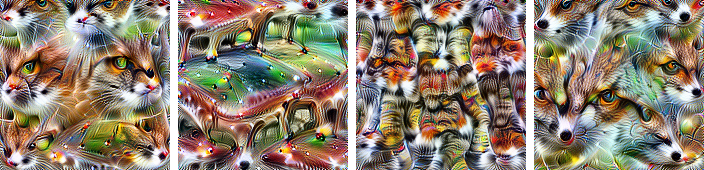
\includegraphics[width=\linewidth]{figures/feature_visualization.png}
    \caption{GoogleNet hálózat 4e inception moduljának egy vizualizációja}
    \label{fig:featurevisualization}
\end{figure}

A hibafüggvény általában arra optimalizál, hogy minél magasabb értéket vegyen fel egy neuron vagy réteg kimenete, ezáltal olyan képet létrehozva amit "érdekesnek talál" a háló.

A kiinduló állapotként gyakran alkalmaznak véletlen bemenetet és tanító példákat is. A tanító példákra valid kritika, hogy nem lehet tudni az eredmény milyen mértékben a háló belső karakterisztikája és milyen mértékben csak a bemenet egy torzítása. Másik probléma, hogy egy kép nem reprezentatív a háló működésére, mert nem csak arra a mintára vagyunk kíváncsiak amire leginkább aktiválódik a vizsgált hálózatrész, hanem azokra is amikre kevésbé reagál, de még fontosnak találja őket. Erre a problémára nem megoldás több véletlen állapotból indítani az optimalizációt, mivel gyakran nagyon hasonló eredmények alakulnak ki. 

A hiba függvény olyan módú változtatása, hogy penalizálja a korábbiakhoz hasonló képeket javít a képek sokszínűségén, de a képek közti különbség számolásnak is vannak korlátai (például azonos minták jelenléte felcserélve nagy távolságot eredményez), ezért így sem lehet konzisztensen előállítani az összes lényeges mintát.

A tulajdonság vizualizáció segít intuíció szerzésében a hálók belső működésével kapcsolatban, ez nagyon értékes mivel a mélyebb megértés segíti a kutatókat. Ezen kívül vizuálisan és érdekesek, ami közelebb hozhatja az embereket a gépi tanuláshoz. Viszont a bevezetőben felvázolt célra nem a legmegfelelőbbek. Ennek oka, hogy maguk az eredmények nehezen értelmezhetőek, ezért ha még tartalmaznak is utalást egy problémára a tanításban, az nehezen lesz megfogható. Továbbá ezek a módszerek nagyrészt specifikusak a háló implementációjára (kivéve ha a kimenetet tekintjük, de annak is megvannak a saját problémái), ezért általános alkalmazásuk nehézkes. Ezen okokból bár ezen a területen is sok érdekes algoritmus létezik, nem tartoznak szorosan ezen dokumentum tematikájához.

\section{Hozzátulajdonítás (attribution)}

Ezen módszer kimenetekhez bemeneti tulajdonságokat tulajdonít, ezáltal mutatva, hogy mely bemenetek fontosak a feldolgozásban. Tulajdonképpen megmagyarázza, hogy egy bemenetnél mire alapozta döntését a modell.






\section{Potenciális előnyök}

\chapter{LIME}\label{ch:lime}

A LIME egy modell-agnosztikus magyarázatgeneráló rendszer. A LIME feloldása \foreignlanguage{english}{Linear Model-Agnostic Expalantions}, melyben a lineáris arra referál, hogy egy lineáris modell a magyarázat. A keretrendszer képes szöveg, kép és egyszerű egy dimenziós vektorként megadott tulajdonságokkal dolgozó modellek magyarázatára. 

\section{Az ideális magyarázó elvárásai}

Legyen most a magyarázatgenerálás célja a tanító adathalmazbeli zajok által létrehozott rossz általánosítás eredményező modell karakterisztikák egyszerűen felismerhetővé tétele. Nem csak a probléma létének felismerése, hanem forrásának beazonosítása is cél, azokban az esetekben is, mikor a probléma nem okoz helytelen kimenetet.

Az egyszerű felismerhetőség egzakt módon nehezen megfogható koncepció. A minimum hogy a területben járatos szakemberek egy magyarázat alapján a modell a példa körüli lokális működésének helyességét viszonylagos biztossággal meg tudják ítélni rövid idő alatt. Hogy a magyarázatok reprezentatívak legyenek a teljes modellre nézve, sok magyarázat kiértékelésére van szükség, ezért a gyors értékelhetőség igénye kritikus fontosságú. A legjobb eredmény eléréséhez kompromisszumra van szükség a magyarázat komplexitása és a kiértékelés időigénye közt.

A LIME rendszer a magyarázatokra intuitív működésük és egyszerűségük miatt lineáris modelleket használ, ezen túl a kiértékelendő magyarázatok számának csökkentése érdekében a submodular pick algoritmust használja.

\section{Lokális magyarázatok}

Egy komplex nem-lineáris modell működése globálisan nem közelíthető egy lineáris modell segítségével, mivel az csak lineárisan szerparálható feladatokat képes megoldani, ahogy az \aref{sec:linszep} szekcióban tárgyalva volt. Viszont az állapottér egy kisebb részét tekintve egy lineáris modell is reprezentatív lehet, ez a lokális közelítés. A lokalitás eléréséhez a lime két módszer kombinációját alkalmazza:

%TODO mekkkora környezetben véges mintavételt?
%a scikit random normal az normál eloszlást csinál?
\begin{itemize}
	\item a magyarázandó példa körül véletlen mintavételezés
	\item a hibafüggvény súlyozása egy $\pi_x (z)$ távolságfüggvénnyel
\end{itemize}

A folytonos tulajdonságok mintavételezése normál eloszlás alapú véletlen számmal történik, aminek értékét a tanító adathalmazból meghatározott értékkészlettel skáláz a rendszer. A kategorikus tulajdonságok esetében pedig a tanító adathalmazból kiszámolt gyakoriságok alapján generált véletlen kategóriával történik. A magyarázandó példát mindig tartalmazza mintavételezéssel létrehozott adathalmazhoz.

A a távolsághoz képest vett súlyozás függvénye

\begin{equation}
    \pi_x (z) = exp\left(\frac{-D(x',z')^2}{\sigma^2}\right),
\end{equation}

ahol $x'$ a magyarázandó példa, $z'$ az $x'$ körüli generált példa, $D$ egy távolságfüggvény ami alkalmazási területenként változhat. Például szövegek esetén koszinusz távolság, képek esetén euklideszi távolság. $\sigma$ pedig egy szélességi paraméter ami megadja, hogy az eseménytér mekkora hányadát fedje le a $\pi$ függvény. $\sigma$ érték alapértelmezetten $|\x'|*0.75$ ($|\x'|$ a bemeneti tulajdonságok száma), de explicit módon is megadható.

\begin{figure}[H]
    \centering
		\begin{tikzpicture}
            \begin{axis} [width=0.6\textwidth,samples=100,xmin=0,xmax=20,xlabel={$D(x',z')$}, ylabel={$\pi(z')$},ylabel style={rotate=-90},ymin=0, ymax=1,domain=0:20, legend entries =  {$\sigma = 1$\\$\sigma=2$\\$\sigma=3$\\},]
                \addplot[mark=none,line width=0.5mm] {e^(-x/1)};
                \addplot[mark=none,densely dashed,line width=0.5mm] {e^(-x/4)};
                \addplot[mark=none,dotted,line width=0.5mm] {e^(-x/9)};
                %\node at (-1.5,0.75) {$f(x) = \cfrac{1}{1+e^{-x}}$};
            \end{axis}
        \end{tikzpicture}
	\caption{Példák súlyozása a magyarázandó példától vett távolság függvényében, három különböző szigma értékre}
\end{figure}

Maga a $g(z')$ magyarázat modell tehát így néz ki:

\begin{equation}
    g(z') = w_g\cdot z'
\end{equation}

és az optimalizálandó hibafüggvény:

\begin{equation}
    L(y,g,\pi_x) = \sum_{z' \in \boldysmbol Z} \pi_x(z')\left(y(z')-g(z')\right)^2 
\end{equation}


\subsection{Értelmezhetőség}

Egy lineáris modell önmagában egyszerűen értelmezhető még laikusok számára is, mivel a menetekhez tartozó súly értelmezhető a tulajdonság fontosságaként. A negatív súlyú tulajdonságok azt is megadják, hogy mely változók jelenléte csökkenti a modell bizonyosságát a prediktált osztályban.

Viszont nagyszámú attribútum esetén egy lineáris modell sem értelmezhető egyszerűen. Nem elvárható, hogy a felhasználó például 1000 paramétert végignézzen. Ráadásul nagy számú paraméter esetén a túltanulás veszélye lineáris modellek esetén is megnő.
Ennek elkerülése végett érdemes maximalizálni a magyarázat által felhasznált tulajdonságok számát, legyen ez a felső korlát $K$. $K$ értéke nem lehet nagyon kicsi, mert fontos tulajdonságok maradhatnak ki, de túl nagy sem lehet, mert az nagyon lassítaná a kiértékelési procedúrát. Ökölszabályként használható a a $K=7-8$ érték, mivel becslések alapján ennyi független dolgot képes az agy egyidőben a rövidtávú memóriában tárolni. 

Erre a problémára a lime több alternatív megoldást is kínál:
\begin{itemize}
    \item iteratív módon hozzáadni a modellt leginkább javító tulajdonságokat
    \item a legnagyobb súlyú értékek választása
    \item LASSO regularizáció
\end{itemize}

Az iteratív kiválasztás minőségi eredményt szolgáltat, de nagyon költséges. Minden tulajdonság hozzáadásánál az összes fennmaradó tulajdonságra be kell tanítani egy modellt, ami $|x| >> K$ esetben közelítőleg $K*|x|$ tanítási folyamatot jelent. Költsége miatt automatikus esetben a LIME $K<6$ esetben használja ezen módszert. 

A legmagasabb súly kiválasztásán alapuló módszer esetén egy modellt tanít a rendszer, majd a súlyokat megszorozza a magyarázandó példa tulajdonságaival, az így kapott értékek közül a K legnagyobbat használja fel a magyarázatban. Ez a módszer nagyon gyors, viszont nem véd a túltanulás ellen. Például egy olyan esetben, ahol bináris tulajdonságok vannak és van egy tulajdonság ami a mintákban csak kevés esetben vesz fel 1 értéket, de az esetben a célváltozó is mindig aktív, ezért a modell nagy súlyt fog hozzárendelni, pedig nem feltétlenül fontos változó. 

A LASSO módszer regularizáció segítségével választja ki a magyarázatba bekerülő tulajdonságokat. A módszer lényege, hogy a felhasznált súlyok abszolútérték-összege növekedését bünteti azzal, hogy egy $\alpha$ skalárral megszorozva hozzáadja a hibafüggvényhez. A LIME rendszer a least angle regression algoritmust használja a LASSO regularizált modell számításához.

\section{Magyarázandó példák kiválasztása}

Véletlenszerűen kiválasztott példák esetén redundánsak lehetnek a magyarázatok. Két magyarázat akkor redundáns, ha azonos okokból történik a predikció, azaz a magyarázatban ugyanazok az attribútumok szerepelnek hasonló súlyokkal. 

A redundancia elkerülésére a LIME a submodular pick algoritmust alkalmazza. Az algoritmus felhasznál egy már létrehozott magyarázat halmazt, mely optimális esetben tartalmazza az összes rendelkezésre álló példa magyarázatát. Ezen példákba beletartoznak a tanító példák is, amik bár pontosság meghatározására túltanulás miatt nem használhatóak, de magyarázatok esetén pont hogy hasznos hogy felszínre hozza a túltanulásból adódó problémákat. Ez az ideális eset futási idő szempontjából gyakran nem elérhető és ha az is, lehetséges hogy egy kisebb számú magyarázatot de jobb minőséget adó algoritmus előnyösebb.

\newcommand{\W}{\ensuremath{\boldsymbol W}}

Legyen \W a magyarázatok mátrixa, melyben minden oszlop egy tulajdonsághoz tartozik, a sorok pedig a magyarázatokhoz. Legyen \W minden eleme nulla, majd a magyarázatokban szereplő tulajdonságokhoz tartozó elemeket állítsuk a hozzá tartozó súly abszolút értékére. Egy tulajdonság jelentőségét jelölje $I$, értéke pedig legyen

\begin{equation}
    I_{j} = \sqrt{\sum_{i=1}^{n} \W_{i,j}}
\end{equation}

Minél nagyobb $I$ érték tartozik egy tulajdonsághoz az algoritmus annál fontosabbnak tartja, hogy azt tartalmazó példa bekerüljön a szűrt magyarázat listába.

Az algoritmus mohó módon kiválasztja azt a magyarázatot, melyben szereplő tulajdonságok $I$ szummája maximális. Ezután a kiválasztott magyarázat tulajdonságainak $I$ értékét nullára állítja, mivel hozzáadott értékkel nem jár ha kétszer is bekerülnek, mivel az redundáns lenne.

Ezen lépésnél van jelentősége annak is, hogy $I$ értéke gyökös, mivel így két kisebb jelentőségű tulajdonság bevételét fontosabbnak tartja az algoritmus, mint egy a másikét ami kétszer fontosabb. Ezáltal több különböző tulajdonság szerepelhet a szűrt listában.

A submodular pick gyors futási időt biztosít de elhanyagol pár tényezőt. Lehetséges, hogy a legfontosabb tényezőkből érdemes szándékosan többet is bevenni, hogy a kiértékelő számára egyértelműbb legyen a tulajdonság fontossága. Természetesen bekerülhet egy tulajdonság több különböző magyarázatba is, de csak akkor ha az a példa más tulajdonság miatt lett kiválasztva. 

Ezen kívül ha már minden tulajdonság bekerült a szűrt halmazba, az algoritmus nem képes több magyarázatot kiválasztani. Ez természetesen egyszerűen orvosolható például az algoritmus újrafuttatásával, ahol a már kiválasztott magyarázatok kikerülnek a bemenetből.



\chapter{Gyakorlati alkalmazás}\label{ch:example}
\section{Ateizmus adathalmaz}



\section{Genetiaki adabázis}

A magyarázatgenerálás sok attribútum esetén a legfontosabb, és ez esetben értékelhető legjobban az tulajdonság kiválasztás pontossága.Ez az adathalmaz 79272 példát és 2400 tulajdonságot tartalmaz, ezért ideális a rendszer szélsőséges attribútumszám esetén nyújtott teljesítményének tesztelésére. A tulajdonságok valós adatokból kerültek ki, de a használt célváltozó mesterségesen generált. A generáló valószínűségi modell paraméterei rendelkezésre állnak, ami a magyarázatok minőségének kiértékelését is lehetővé teszi.

Az adatbázis kategorikus formátumú genetikai változókból áll. Minden genetikai változó három értéket vehet fel:
\begin{itemize}
	\item  0 ha mindkét szülőtől kapott nukleotid azonos és a populációban gyakrabban megfigyelt értéket veszi fel
	\item 1 ha a szülőktől különböző nukleotidok származnak
	\item 2 ha a szülőktől azonos, a populációban ritkábban előforduló nukleotid van jelen
\end{itemize}
A nukleotidok gyakorisága az adatbázisban megfigyelt eloszlás alapján van meghatározva. Mikor mindkét variáció jelen van nem lehet tudni, hogy melyik a domináns, ezért az 1 kódolással, mintegy köztes érték van reprezentálva. Ezen kívül jelen van még három nem genetikai változó is, a stressz, a nem és a kor. Egy valós célváltozó esetén ezeknek fontos szerepük lenne mert szabályozzák a génexpressziót, de mivel mesterséges a célváltozó, nincs külön szemantikus jelentésük. A kor és stressz is kategorikus módon vannak megadva, három értéket vehetnek fel, amik korosztályoknak és stressz kategóriáknak felelnek meg.
	
\section{Modell optimalizálás folyamata}

A szélsőséges számú tulajdonság problémákat jelent a tanítás szempontjából, megoldásuk pedig egyedi megoldásokat kíván.

\subsection{Négyzetes paraméter szám}
	
Egy lineárisan nem szeparálható probléma megoldásához legalább egy rejtett rétegre szükség van. Ez a rejtett réteg nem lehet túl kis méretű, mivel az jelentősen csökkentené az információt amivel a további rétegek dolgozhatnak.
Ezért elengedhetetlen, hogy az első rejtett rétegnek legalább százas nagyságrendben legyen a neuronszáma. Mivel sűrű kötés esetén a súlyok száma a szomszédos rétegek neuronszámának a szorzata, ez nagy súlyszámot okoz. Például 512 neuronos réteg és 2400 bemeneti tulajdonság esetén $2400*512 = 23.5M$ súly van, ami például 10\%-a a GoogleNet által használtnak, pedig az képek több mint 100 kategóriás klasszifikációjára lett kifejlesztve. 2400 tulajdonság pedig genetikai adatbázisok esetén kevésnek is számít, 24000 változó esetén a súlyok száma már 12 millió, ami rengeteg kapacitást ad a háló számára túltanuláshoz.

\subsection{Lokális kötésű első réteg}

Kézenfekvő megoldás a négyzetes paraméterszámra olyan struktúra alkalmazása, melynek lineáris a paraméterszáma. Ha a réteg minden neuronjába konstans számú variáns futna be, nagy tulajdonságszámnál sem következne be paraméterszám robbanás. Ezt valósítja meg a lokális kötésű réteg, melyben minden neuron a bemeneti variánsoknak egy csúszó-ablak által meghatározott részét kapja bemenetként. Hasonló módon egy 1 dimenziós  konvolúciós réteghez, azzal a különbséggel, hogy az ablak minden pozíciójában változnak a súlyok.

\begin{figure}[H]
    \centering
	\begin{tikzpicture}[circle]
	
	% first layer neurons
	\node[line width=0.5mm,draw,minimum size=0.5cm] (a) at (0cm,0cm) {};
	\node[line width=0.5mm,draw,minimum size=0.5cm] (b) [below=0.3cm of a] {};
	\node[line width=0.5mm,draw,minimum size=0.5cm] (c) [below=0.3cm of b] {};
	\node[line width=0.5mm,draw,minimum size=0.5cm] (d) [below=0.3cm of c] {};
	\node[line width=0.5mm,draw,minimum size=0.5cm] (e) [below=0.3cm of d] {};
	\node[line width=0.5mm,draw,minimum size=0.5cm] (f) [below=0.3cm of e] {};
	\node[line width=0.5mm,draw,minimum size=0.5cm] (g) [below=0.3cm of f] {};
	
	%second layer neurons 
	\node[line width=0.5mm,draw,minimum size=0.5cm,red] (aa) at (3cm,-0.85cm) {};
	\node[line width=0.5mm,draw,minimum size=0.5cm,green] (bb) [below=1.15cm of aa] {};
	\node[line width=0.5mm,draw,minimum size=0.5cm,blue] (cc) [below=1.15cm of bb] {};
	
	%connections of aa
	\draw[line width=0.5mm,red] (a) -- (aa);
	\draw[line width=0.5mm,red] (b) -- (aa);
	\draw[line width=0.5mm,red] (c) -- (aa);
	%connections of bb
	\draw[line width=0.5mm,green] (c) -- (bb);
	\draw[line width=0.5mm,green] (d) -- (bb);
	\draw[line width=0.5mm,green] (e) -- (bb);
	
	%connections of cc
	\draw[line width=0.5mm,blue] (e) -- (cc);
	\draw[line width=0.5mm,blue] (f) -- (cc);
	\draw[line width=0.5mm,blue] (g) -- (cc);
	
	\end{tikzpicture}
	\caption{Sematikus ábrája egy lokális kötésű rétegnek, aminek ablakszélessége 3 stride-ja pedig 2}
\end{figure}

Ezzel a megoldással szabályozható a paraméterek száma, úgy hogy közben az első rejtett réteg neuronszáma is tetszőlegesen állítható. A struktúra önmagában nem biztosítja, hogy minden bemenet azonos számú neuronba fusson be, de azzal a megszorítással hogy a stride osztója kell legyen az ablak szélességnek, egyszerűen biztosítható.

\begin{figure}[H]
    
		\begin{subfigure}{\linewidth}
		\centering
			\begin{tikzpicture}
               \begin{axis}[width=0.5\textwidth,xmin=0,xmax=200,every axis plot/.append style={thick},legend entries =  {tanító hiba\\validációs hiba\\},legend pos=north west]
                \addplot+[mark=none] table [x=epochs, y=training, col sep=comma] {data/dense.csv};
                \addplot+[mark=none] table [x=epochs, y=validation, col sep=comma,mark=none] {data/dense.csv};
        \end{axis}
        \begin{axis}[at={(0.53\linewidth,0)},width=0.5\textwidth,xmin=0,xmax=200,every axis plot/.append style={thick},ylabel style={rotate=-90},legend entries =  {tanító hiba\\validációs hiba\\}]
        \addplot+[mark=none] table [x=epochs, y=training, col sep=comma] {data/local.csv};
        \addplot+[mark=none] table [x=epochs, y=validation, col sep=comma,mark=none] {data/local.csv};
        \end{axis}
            \end{tikzpicture}
		\end{subfigure}
	\caption{Egyébként azonos konfigurációk bal oldalon sűrű, jobb oldalon lokális kötésű első rejtett réteggel  \label{densevslocal}}
\end{figure}

\Aref{densevslocal} ábrán látható, hogy 512 neuron tartalmazó sűrű kötésű első réteg esetén a milliós nagyságrendű paraméterszám egyszerűvé teszi a hálózatnak, hogy teljesen rátanuljon a tanítómintákra. A kétszázadik epoch környékén a tanító adatokon vett hiba effektíve nulla, 

\subsection{Tanítás nehézségei}

A nagy számú tulajdonság szükségszerűen megnöveli az esélyét, hogy egy tulajdonság véletlen alapján korrelációt mutasson a célváltozóval. Ha a tulajdonságok egy részhalmazának tetszőleges függvényét vesszük, méginkább nő valószínűsége, hogy létezik olyan ami a véletlen folytán mutat nagy korrelációt. Ezen körülmények nagyon egyszerűvé teszik a túltanulást. A hiperparaméter optimalizálásnak fő nehézsége a túltanulás és a hálózat túlzott lekorlátozása közti egyensúly megtalálása volt.

\subsection{Túltanulás elleni eszközök}

A tanítás során a túltanulásának fő eszközei ezek a paraméterek voltak:
\begin{itemize}
    \item batch méret
    \item dropout
    \item paraméterszám
    \item réteg struktúra
\end{itemize}

A paraméterek beállítását az is nehezíti, hogy több aspektusban is változtathatják a háló viselkedését, ami más paraméterek egyidejű hozzáigazítását is megköveteli. Például a batch méret növelése nagyobb tanulási sebességet igényel és csökkenti a dropout igényét is.

A batch méretnek is lehet hatása a túltanulásra, mivel a túltanulás lényegében úgy jön létre, hogy a háló a konkrét példákat tanulja meg. De ha biztosítjuk, hogy csak olyan lépést tehet az algoritmus, ami egyszerre sok példára csökkenti a hibát, nehéz egyedi példákat azonosító függvényt létrehozni.

A dropout lényege, hogy egy réteg bemenetein megadott valószínűséggel nullázódnak a tulajdonságok, így nehezíti, hogy a háló beazonosítsa hogy melyik már korábban látott példát kapta bemenetként. Hátránya viszont, hogy a keresett összefüggés megtalálását is nehezíti. A dropout alkalmazható bármely rétegre, de a tanítás során csak a bemeneti rétegre lett alkalmazva.

A paraméterek száma felfogható a hálózat memóriája méretének is, amiből ha a keresett összefüggés megtanulásához szükségesen túl több van, a háló potenciálisan tanító példák megtanulására fordíthatja a kapacitást. Az hogy mennyi a minimális szükséges paraméter gyakorlatilag nem számítható. Léteznek elméletileg bizonyított felső korlátok, egy tetszőleges függvényt leíró neurális hálózat paraméterszámára, de olyan magas becslést adnak, hogy gyakorlatban nem használhatóak. Intuitív módon viszont becsülhető, hogy mekkora méret ami már szinte biztos, hogy fölösleges. Jó becslési alap a példák és paraméterek aránya, például ha minden tanító példára 100-1000 paraméter jut, az több mint valószínű hogy szükségtelen.

\subsection{Optimalizálás folyamata}




\section{Magyarázat generálás folyamata}

\section{Konklúzió}



%kategorikus változók jobb perturbálása
%submodualr pick módosítás
%least angle regression futásidő optimalizálás

% Acknowledgements
%~~~~~~~~~~~~~~~~~~~~~~~~~~~~~~~~~~~~~~~~~~~~~~~~~~~~~~~~~~~~~~~~~~~~~~~~~~~~~~~~~~~~~~
%----------------------------------------------------------------------------
\chapter*{\koszonetnyilvanitas}\addcontentsline{toc}{chapter}{\koszonetnyilvanitas}
%----------------------------------------------------------------------------

Ez nem kötelező, akár törölhető is. Ha a szerző szükségét érzi, itt lehet köszönetet nyilvánítani azoknak, akik hozzájárultak munkájukkal ahhoz, hogy a hallgató a szakdolgozatban vagy diplomamunkában leírt feladatokat sikeresen elvégezze. A konzulensnek való köszönetnyilvánítás sem kötelező, a konzulensnek hivatalosan is dolga, hogy a hallgatót konzultálja.


% List of Figures, Tables
%~~~~~~~~~~~~~~~~~~~~~~~~~~~~~~~~~~~~~~~~~~~~~~~~~~~~~~~~~~~~~~~~~~~~~~~~~~~~~~~~~~~~~~
%\listoffigures\addcontentsline{toc}{chapter}{\listfigurename}
%\listoftables\addcontentsline{toc}{chapter}{\listtablename}


% Bibliography
%~~~~~~~~~~~~~~~~~~~~~~~~~~~~~~~~~~~~~~~~~~~~~~~~~~~~~~~~~~~~~~~~~~~~~~~~~~~~~~~~~~~~~~
\addcontentsline{toc}{chapter}{\bibname}
\bibliography{bib/mybib}


% Appendix
%~~~~~~~~~~~~~~~~~~~~~~~~~~~~~~~~~~~~~~~~~~~~~~~~~~~~~~~~~~~~~~~~~~~~~~~~~~~~~~~~~~~~~~
%----------------------------------------------------------------------------
\appendix
%----------------------------------------------------------------------------
\chapter*{\fuggelek}\addcontentsline{toc}{chapter}{\fuggelek}
\setcounter{chapter}{\appendixnumber}
%\setcounter{equation}{0} % a fofejezet-szamlalo az angol ABC 6. betuje (F) lesz
\numberwithin{equation}{section}
\numberwithin{figure}{section}
\numberwithin{lstlisting}{section}
%\numberwithin{tabular}{section}

%\label{page:last}
\end{document}
